\documentclass[
	11pt, 
	a4paper, 
	twoside, 
	openright, 
	titlepage=firstiscover, 
	numbers=noenddot, 
	BCOR=12mm,
	headsepline,
	footsepline,
	toc=listof,
	toc=bibliography
	]{scrbook}

%%%%%%%%%%%%%%%%%%%%%%%%%%%%%%%%%%%%%%%%%%%%%%%%%%%%%%%%%%%%%%%%
%%
%% 1. Configure Document
%%
%%%%%%%%%%%%%%%%%%%%%%%%%%%%%%%%%%%%%%%%%%%%%%%%%%%%%%%%%%%%%%%%

%todo: Configure Document
\let\cleardoublepage\clearpage
\def\doclanguage{english} %english, german, ngerman	
\def\doctitle{Smart Contract Development with JASON BDI Agents}
\def\doctype{Master's Thesis}
\def\docdate{\today}
\def\authorname{Mostakim Mullick}
\def\authorbirthday{20.02.1998}
\def\authorbirthplace{Hooghly, West Bengal, India}
\def\professor{Prof. Dr. Uwe Aßmann}
\def\supervisors{Prof. Dr. Uwe Aßmann\\Orçun Oruç, M.\,Sc. }
\def\reviewers{Prof. Dr. Uwe Aßmann\\Dr.-Ing. Sebastian Götz }
%%%%%%%%%%%%%%%%%%%%%%%%%%%%%%%%%%%%%%%%%%%%%%%%%%%%%%%%%%%%%%%%
%%
%% 2. Take a Look at the Following Predefined Commands
%%
%%	- encoding is utf8 and does not require entities for ä/ö/ü/ß
%%	- generate the document using XeLaTeX instead of pdfLaTeX 
%%	- and Biber engine instead of BibTeX
%%	- Ensure, your TeX distribution is up to date!
%%
%%	- BIB-File is located at includes/bibliography.bib
%%	- abbreviations supported (includes/acronyms.tex)
%%	- multiple columns supported (multicol)
%%	- URLs supported (url)
%%
%%	- definitions and formulae supported
%%		USAGE:
%%		\begin{definition}[<term>]	| \begin{formula}[<term>]
%%		\label{def:<term>}			| \label{for:<term>}
%%			<definition text>		| 	 <formula text>
%%		\end{definition}				| \end{formula}
%%
%%	- listings supported (listings)
%%		USAGE:
%%		inline:
%%			\begin{lstlisting}[caption=<caption>, label=lst:<label>]
%%				<YOUR CODE HERE>
%%			\end{lstlisting}
%%		include:
%%			\lstinputlisting[language=Python]{source_filename.py}
%%
%%	- predefined commands for TODOs
%%		USAGE:
%%		\todo{This is a sandbox todo.}
%%		\todo[Wow]{This as well with own labeling.}
%%		\enhancement{This is an enhancement.}
%%
%%%%%%%%%%%%%%%%%%%%%%%%%%%%%%%%%%%%%%%%%%%%%%%%%%%%%%%%%%%%%%%%

%to do: Look into the available commands

% language constants
\def\english{english}
\def\german{german}
\def\ngerman{ngerman}
\def\true{true}
\def\false{false}

% DOCUMENT LAYOUT SETUP (Encoding, Language, Fonts, Page Setup) 
% 
\usepackage[utf8]{inputenc}	% Encoding
\usepackage{fontspec} % New font management (requires XeLaTeX)
\usepackage{lmodern} % Use (improved) font Latin Modern
% Custom Fonts
\linespread{1.05} % Adjust line spacing, depending on what font you use
\setmainfont{Lora}[
	Path 			= includes/fonts/Lora/ ,
	Extension		= .ttf ,
	UprightFont		= *-Regular ,
	BoldFont		= *-Bold ,
	ItalicFont		= *-Italic ,
	BoldItalicFont	= *-BoldItalic ,
	Scale			= .93 % Adjust font size
	 ]
\setsansfont{Lato}[
	Path 			= includes/fonts/Lato/ ,
	Extension		= .ttf ,
	UprightFont		= *-Regular ,
	BoldFont		= *-Bold ,
	ItalicFont		= *-Italic ,
	BoldItalicFont	= *-BoldItalic ]
\setmonofont{FiraCode}[
	Path 			= includes/fonts/FiraCode/ ,
	Extension		= .otf ,
	UprightFont		= *-Regular ,
	BoldFont		= *-Bold ,
	Scale			= MatchLowercase ]	

\ifx\doclanguage\english
		\usepackage[english]{babel}
\fi
\ifx\doclanguage\german
		\usepackage[german]{babel}
\fi
\ifx\doclanguage\ngerman
		\usepackage[ngerman]{babel}
\fi

\usepackage[left=30mm,right=20mm,top=30mm,bottom=40mm]{geometry} % Page setup

\usepackage[
	pdftoolbar=true,
	bookmarksopen,
	bookmarksnumbered=false,
	bookmarksopenlevel=1,
	pdfdisplaydoctitle,	
    colorlinks,
    citecolor=black,
    filecolor=black,
    linkcolor=black,
    urlcolor=black
]{hyperref} % Linking within PDF

% FORMAT CONTENT
\usepackage{graphicx} % Graphics options like scale

\usepackage[margin=10pt,font=small,labelfont=bf,labelsep=endash]{caption} % Nicer caption layouts

\usepackage{enumitem} % Customise enumeration formats
	% USAGE:
	%	\begin{enumerate}[label=\lbrack\arabic*\rbrack,start=1]
	%		\item Bla --> (creates [1] Bla)
	%	\end{enumerate}
	%
	%	\begin{enumerate}[label=\lbrack\arabic*\rbrack,resume]
	%		\item Bla --> (creates [2] Bla)
	%	\end{enumerate}
	
\usepackage{multicol} % Introduce multi column content
	% USAGE:
	% \begin{multicols}{<number>}
	% 	<multicolumn text>
	% \end{multicols}

\usepackage{url} % Insert clickable URLs
	% USAGE:
	% \url{http://www.google.com}

% PROVIDE CONTENT

\usepackage[printonlyused,withpage]{acronym} % Manage abbreviations
	% USAGE:
	% Create abbreviations in acronyms.tex this way...
	% 	\acro{POSF}{Partly Open Software Family}
	% 	\acroplural{POSF}[POSFs]{Partly Open Software Families}
	% Call abbreviations anywhere in the document this way...
	% 	\ac{abbr.}         % default:	full at first call, short (abbr.) else
	% 	\acs{abbr.}        % short: 	abbr.
	% 	\acf{abbr.}        % full: 	abbreviation (abbr.)
	% 	\acl{abbr.}        % long: 	abbreviation
	% for plural forms, add a -p: \acp, \acsp, \acfp, \aclp
	
\usepackage{blindtext} % Allow blind text
	% USAGE:
	% \blindtext[4] typesets blind text with 4 repetitions
	% \Blindtext[2][3] typesets blind text with 2 paragraphs and 3 rep.

%======================================================================== BIBLIOGRAPHY

\usepackage[
	backend=biber,
	style=alphabetic,
	maxbibnames=50,
	isbn=false,
	backref=true,
	backrefstyle=two+
]{biblatex} % User Biber and BibLaTeX

\bibliography{includes/bibliography}

%======================================================================== THEOREMS

\usepackage{mdframed} % Allows framed and coloured environments
\usepackage{thmtools} % Allows Theorem definitions and lists

\mdfdefinestyle{guidelinestyle}{
%  linecolor=black,					% STYLE 1 (boxed with grey title)
%  linewidth=.8pt,
%  frametitlerule=true,
%  frametitlefont=\sffamily\bfseries,
%  frametitlebackgroundcolor=codebackground,
%  innertopmargin=\topskip,
  frametitlealignment=\center,		% STYLE 2 (lines top, separator, bottom)
  frametitlefont=\normalfont,
  frametitlerule=true,
  rightline=false,
  leftline=false,
  linewidth=.8pt,
  frametitlerulewidth=.4pt
}

\makeatletter
\define@key{thmdef}{mdthm}[{}]{%
\thmt@trytwice{\def\thmt@theoremdefiner{\mdtheorem[#1]}}{}}
\makeatother

\declaretheorem[
	mdthm={style=guidelinestyle},
	%numberwithin=chapter
]{definition}% <environment name>
\makeatletter
\def\ll@definition{% <environment name>
  \protect\numberline{\csname the\thmt@envname\endcsname}
  \ifx\@empty\thmt@shortoptarg
    \thmt@thmname
  \else
    \thmt@shortoptarg
  \fi}
\makeatother
	% USAGE:
	%\begin{definition}[<term>]
	%\label{def:<term>}
	%	<definition text>
	%\end{definition}
	
\declaretheorem[
	mdthm={style=guidelinestyle},
	%numberwithin=chapter
]{formula}% <environment name>
\makeatletter
\def\ll@formula{% <environment name>
  \protect\numberline{\csname the\thmt@envname\endcsname}
  \ifx\@empty\thmt@shortoptarg
    \thmt@thmname
  \else
    \thmt@shortoptarg
  \fi}
\makeatother
	% USAGE:
	%\begin{formula}[<term>]
	%\label{for:<term>}
	%	<formula text>
	%\end{formula}


%======================================================================== LISTINGS

\usepackage{listings} % add source code inclusion opportunity

\lstset{
	basicstyle=\footnotesize\ttfamily,
	commentstyle=\color{tudgreen2}\ttfamily,
	keywordstyle=\bfseries\color{tudblue2},
	captionpos=b,
	language=Java,
	morekeywords={Set, Group, Feature, FeatureModel, Constraint}, 
	numbers=left,  
	numberstyle=\bfseries\ttfamily,
	stepnumber=1, 
	numbersep=5pt,
	tabsize=2,
	texcl=false,
	mathescape=true,
	frame=single,
	framexleftmargin=12pt,
	framextopmargin=1pt,
	framexbottommargin=1pt,
	framexrightmargin=4pt,
	backgroundcolor=\color{codebackground},
	showspaces=false,
	showstringspaces=false,
	numberbychapter=true
}
	% USAGE:
	% inline:
	%	\begin{lstlisting}[caption=<caption>, label=lst:<label>]
	%		<YOUR CODE HERE>
	%	\end{lstlisting}
	% include:
	%	\lstinputlisting[language=Python]{source_filename.py}

%======================================================================== COLOURS

\usepackage[usenames, dvipsnames, svgnames, table]{xcolor} % Manage colours

\xdefinecolor{tudblue}{HTML}{0B2A51}
\xdefinecolor{tudblue2}{HTML}{0059A3}
\xdefinecolor{tudpurple}{HTML}{51297F}
\xdefinecolor{tudpurple2}{HTML}{811A78}
\xdefinecolor{tudgreen}{HTML}{007A47}
\xdefinecolor{tudgreen2}{HTML}{22AD36}
\xdefinecolor{tudorange}{HTML}{E87B14}
\xdefinecolor{codebackground}{rgb}{0.96, 0.96, 0.96}
	% USAGE:
	% \textcolor{tudblue}

%======================================================================== TODOs
%-TODO Tag with optional comment
%(#1: comment) #2: affected region
\newcommand{\todo}[2][TODO]{\textbf{\textcolor{tudpurple2}{[#1]} \textcolor{tudorange}{#2}}}
%-ENHANCEMENT Tag
\newcommand{\enhancement}[1]{\textcolor{tudpurple2}{[Enhancement]} \textcolor{tudblue2}{#1}}
	% USAGE:
	% \todo{This is a sandbox todo.}
	% \todo[Wow]{This as well with own labeling.}
	% \enhancement{This is an enhancement.}






\begin{document}
\pagenumbering{gobble}

	\newgeometry{margin=1in, top=2.5in}

\begin{titlepage}
% front page

\begin{center}

	{\large
		\doctype\relax
	}
	
	\vspace{.5cm}
	
	{\huge \bfseries \sffamily
		\doctitle\relax
		\par
	}
	
	\vspace{1cm}
	
	\ifx\doclanguage\english
		submitted by
	\fi
	\ifx\doclanguage\german
		eingereicht von
	\fi
	\ifx\doclanguage\ngerman
		eingereicht von
	\fi
	
	\vspace{.5cm}
	
	\textbf{\authorname} \\
	\ifx\doclanguage\english
		born
	\fi
	\ifx\doclanguage\german
		geboren am
	\fi
	\ifx\doclanguage\ngerman
		geboren am
	\fi
	\authorbirthday{} in \authorbirthplace

	
	\vspace{1.5cm}
	
	{\Large Technische Universität Dresden}
	
	\vspace{.5cm}
	
	\ifx\doclanguage\english
		Faculty of Computer Science \\
		Institute of Software and Multimedia Technology \\
		Chair of Software Technology

	\fi
	\ifx\doclanguage\german
		Fakultät Informatik \\
		Institut für Angewandte Informatik \\
		Lehrstuhl Mensch-Computer-Interaktion

	\fi
	\ifx\doclanguage\ngerman
		Fakultät Informatik \\
		Institut für Angewandte Informatik \\
		Lehrstuhl Mensch-Computer-Interaktion

	\fi
	
	\vspace{1.0cm}
	
	
\includegraphics[scale=.75]{includes/figures/tu_logo}
	
	\vspace{.5cm}
\end{center}

	\noindent
	\ifx\doclanguage\english
		Supervisors: \\
	\fi
	\ifx\doclanguage\german
		Betreuer: \\
	\fi
	\ifx\doclanguage\ngerman
		Betreuer: \\
	\fi
	\supervisors
	
	\vspace{.5cm}
	
	\noindent
	\ifx\doclanguage\english
		Reviewers: \\
	\fi
	\reviewers
	
	\vspace{.5cm}
	
	\noindent
	\ifx\doclanguage\english
		Professor: \\
	\fi
	\ifx\doclanguage\german
		Hochschullehrer: \\
	\fi
	\ifx\doclanguage\ngerman
		Hochschullehrer: \\
	\fi
	\professor
	
	\vspace{1.5cm}
	
	\noindent
	\ifx\doclanguage\english
		Submitted
	\fi
	\ifx\doclanguage\german
		Eingereicht am
	\fi
	\ifx\doclanguage\ngerman
		Eingereicht am
	\fi
	\docdate


% Add PDF Meta Data
\hypersetup{
		pdftitle={\doctitle},
		pdfauthor={\authorname},
		pdfsubject={\doctype}
	}

\end{titlepage}

\restoregeometry

	%todo: Include thesis task description here
	% You got it from your supervisor. Scan the document and
	% include it as full-page PDF here. If your task description
	% is larger than 3 pages, consider putting it in the appendix 
	% instead.
	
	% Confirmation
\ifx\doclanguage\english
	\chapter*{Confirmation}
	I confirm that I independently prepared this thesis with the title 
	\emph{\doctitle}
	and that I used only the references and auxiliary means indicated in the thesis.

\fi
\ifx\doclanguage\german
	\chapter*{Erklärung}
	Ich erkläre, dass ich die vorliegende Arbeit mit dem Titel 
	\emph{\doctitle}
	selbständig unter Angabe aller Zitate angefertigt und dabei ausschließlich die aufgeführte Literatur und genannten Hilfsmittel verwendet habe.
\fi
\ifx\doclanguage\ngerman
	\chapter*{Erklärung}
	Ich erkläre, dass ich die vorliegende Arbeit mit dem Titel 
	\emph{\doctitle}
	selbständig unter Angabe aller Zitate angefertigt und dabei ausschließlich die aufgeführte Literatur und genannten Hilfsmittel verwendet habe.
\fi

\vspace{1.5cm}

\noindent
Dresden, \docdate

\vspace{3.0cm}

\noindent
\authorname

 %todo: Sign the confirmation
\pagenumbering{Roman}
	%todo: Write an abstract
	% Confirmation
\ifx\doclanguage\english
\chapter*{Abstract}

   Blockchain use has skyrocketed in recent years, and various blockchains customized to specific use cases have emerged. The blockchain technology stack has grown tremendously since Bitcoin, the first true blockchain application. One of the most essential blockchain uses is smart contracts. Most present smart contract systems presume that when contracts are executed over a network of decentralized nodes, the majority's decision can be trusted. However, we have seen that people associated with a smart contract may intentionally take steps to manipulate contract execution in order to improve their own gains. To solve this issue, we suggest an agent model as the underlying mechanism for contract execution over a network of decentralized nodes and a public ledger, and we analyze the prospect of prohibiting users from influencing smart contract execution.
    
    Numerous research and application sectors are being impacted by the blockchain technology and idea, and as a result, many see this as an opportunity to find new solutions to old issues or reap innovative advantages. Several writers in the agent community are proposing their own mix of agent-oriented technology with blockchain to address both old and new difficulties. This thesis paper aims to define the prospects, factors to consider, and analyzing information about the content for combining agents with blockchain.
    
     
	\tableofcontents
	
\pagenumbering{arabic} 

	%todo: Write you thesis content
	
\ifx\doclanguage\english
\chapter{Introduction}

The term \textit{"agent"} is commonly used these days. This applies to both \ac{AI} and fields outside of it, such as databases and automated manufacturing. Despite growing in popularity, the phrase has been employed in so many different contexts that it has lost all meaning when not connected to a certain understanding of agenthood. The terminology "agent" is most frequently used in the context of  \ac{AI} to describe an object that operates constantly and autonomously in a context that also contains other processes and agents.
Perhaps this is the single characteristic that all practitioners of the word in \ac{AI} agree upon. Although the definition of "autonomy" is vague, it is generally understood to suggest that the behaviors of the agents do not need ongoing human direction or interference. Additional presumptions are frequently made about the environment, such as that it is physical and mostly unpredictable.

\vspace{.5cm}

Agents are frequently assumed to be robotic agents, in which case additional problems including sensory input, motor control, and time constraints are stated. Finally, agents are frequently perceived as "high-level." Although this meaning is somewhat nebulous, many people use some variation of it to separate agents from other pieces of hardware or software. The "high level" is exhibited by symbolic representation and/or cognitive-like skills. Agents may be "informable," have symbolic planning in addition to stimulus-response rules, and even be able to speak. This meaning is not universally assumed in \ac{AI}, so clearly, the concept of agenthood in \ac{AI} is far from clear. As a result, We should be explicit about what we mean when we use the term "agent," which is as follows: An entity whose state is seen to be composed of mental elements including beliefs, capabilities, decisions, and commitments is referred to as an agent. These elements are precisely specified and roughly correspond to their equivalents from common sense. Therefore, according to this perspective, an agent only exists in the programmer's head. Any hardware or software component only qualifies as an agent if its analysis and management have been done in this way.

\vspace{.5cm}

In latest years, there has been a lot of interest in the research of computational agents that can behave rationally. The architecture of systems required to conduct high-level management and control activities in complex dynamic situations is becoming increasingly important in the commercial world. Air traffic control, telecommunications networks, commercial operations, space spacecraft, and medical services are examples of such systems. Experience with using traditional software methodologies to design such systems has revealed that they are extremely complicated and costly to build, validate, and sustain. Agent-oriented systems, which are based on a fundamentally different perspective of computational entities, provide opportunities for a qualitative shift in this stance. 

\vspace{.5cm}

One such architecture views the system as a rational agent with particular mental attitudes of Belief, Desire, and Intention (\ac{BDI}), reflecting, respectively, the informational, motivating, and deliberative states of the agent. When deliberation is subject to resource constraints, these mental attitudes govern the system's behavior and are crucial for obtaining adequate or optimal performance.

\vspace{.5cm}

\ac{BDI} agents can be considered for both a formulation of a theory and a practical design standpoint. However, there is still a significant discrepancy between theory and practice. The complication of theorem-proving or model-checking in these expressive specification logics has been the primary cause for this. As a result, \ac{BDI} systems that have been deployed have tended to employ the three primary attitudes as data structures rather than modal operators. \textit{AgentSpeak(L)} is a generalization of one of the implemented \ac{BDI} systems that allows agent programs to be developed and processed in the same way as a horn-clause rationale programs.

\vspace{.5cm}

It is a language of programming based on a limited first-order language with events and actions. The programs created in AgentSpeak(L) govern the agent's behavior (i.e., its interaction with the environment). The agent's beliefs, desires, and intentions are not explicitly stated as modal formulae. Instead, as designers, one may attribute these ideas to AgentSpeak(L) agents. The agent's present belief state may be considered as a model of itself, its environment, and other agents; states that the agent seeks to bring about based on external or internal stimuli can be viewed as desires; and the adoption of programs to meet such stimuli can be viewed as intents.

\vspace{.5cm}

It is a language of programming based on a limited first-order language with events and actions. The programs created in AgentSpeak(L) govern the agent's behavior (i.e., its interaction with the environment). The agent's beliefs, desires, and intentions are not explicitly stated as modal formulae. Instead, as designers, one may attribute these ideas to AgentSpeak(L) agents. The agent's present belief state may be considered as a model of itself, its environment, and other agents; states that the agent seeks to bring about based on external or internal stimuli can be viewed as desires; and the adoption of programs to meet such stimuli can be viewed as intents. 

\vspace{.5cm}

It is therefore easy to design an agent capable of controlling its surroundings on its own, but this becomes troublesome when the environment is shared by more than one agent. AgentSpeak(L) is extended by languages such as jason and \ac{ASTRA}. They could be used to implement that language's operational semantics and provide a foundation for the development of \ac{MAS} with different user-customizable features.

\vspace{.5cm}

The implementation of these agents in specialized fields would be helpful when discussing about the agents' ability to communicate utilizing AgentSpeak(L). One of the most significant areas will be supply chain management, where we may assign roles to various agents such as manufacturers, wholesalers, and retailers.It seems sense that whenever agents interact, there will be a transaction, and that transaction should be recorded. Rather than keeping these interactions in databases or spreadsheets, it will be perfect for storing them in smart contracts, which can be inspected for tracking or future references. 

\vspace{.5cm}

The concept of \textit{smart contracts}, or computer protocols intended to automatically facilitate, authenticate, and implement the negotiation and application of digital contracts without the need for centralized authorities, has been revived in recent years has resulted of the rapid development of cryptocurrencies and the \ac{BCT} that underpins them. Smart contracts have been incorporated into popular blockchain-based development platforms like Ethereum and Hyperledger. They have a wide range of potential application areas in the globalised era and intelligent sectors of the economy, including financial sector, management, healthcare, and Internet of Things, among many others.

\vspace{.5cm}

The combination of the agent and blockchain domains appears to be effective. In order to study the operation, compatibility, and behavior pattern of smart contracts with agents, some work has been done in the area of integrating agents with smart contracts.

\vspace{.5cm}

In this thesis, a \textbf{\textit{Smart contract development with jason \ac{BDI} Agents}} is presented. An environment that will show off several agents, allowing agents throughout the supply chain—namely, manufacturers, retailers, and wholesalers—to communicate with one another utilizing a primary agent. This ecosystem will also make it possible to maintain relationships between agents, store transactions using smart contracts and offer a hash for each transaction that may be used to examine further information.


\section{Motivation}

The blockchain is having an increasing influence on a variety of research and application fields, from distributed computing and storage to supply chain management and healthcare accountability. In fact, there are many distinct use cases where the promise of supplying a secure and fault-tolerant ledger that mutually untrusted parties may use to monitor computations and interactions completely dispersed and decentralized without the need for a central authority is intriguing. 

\vspace{.5cm}

The agent community is no different; it began expressing interest in the opportunities presented by the blockchain to either solve long-standing problems (such as trust management in open systems, accountability of actions for liability, among others), or to take advantage of expected benefits to endow a system with new properties (such as novel infrastructures for \ac{MAS}, trustworthy coordination).

\vspace{.5cm}

Smart contracts play a critical role in enabling the blockchain to function as a general-purpose distributed computing engine while retaining its core properties of security, trust, and fault-tolerance, and they actually extend their reach to cover computations other than data storage and management.

\vspace{.5cm}
The convergence of the agent and blockchain worlds appears to be promising: Agents are distributed autonomous entities whose interactions should be managed and mediated in trustworthy ways; blockchains and smart contracts, on the other hand, are trust-sensitive mechanisms for mediating and managing interactions.

\section{Our contributions}

The contribution of the paper are as follows:

\begin{itemize}

    \item We demonstrate and analyze the aspects of \ac{MAS}-\ac{BCT} created by integrating agents with smart contracts, as well as the implications for agent-oriented practice and blockchain. The primary goal was to utilize AgentSpeak(L) to program agents and store their interactions using smart contracts.
    
    \item  The fundamental concept was to construct \ac{MAS} using jason, an extension of AgentSpeak(L), and smart contracts using Solidity and integrating them together.
    
    \item Our research enabled the usage of jason with both the Python interpreter and Java. As an alternative to jason, we also tested using \ac{ASTRA}. Because Java was the prior implementation language, \ac{ASTRA}'s type system is based on it. By using a comparable type system, translating between \ac{ASTRA} and Java is made easier and more clear. Vyper was also taken under consideration for Smart contracts while switching from Java to Python, but was later abandoned owing to some of its drawbacks.
    
\end{itemize}

In order to integrate them, we conducted extensive study while doing that. When choosing a programming language to integrate agents written in agentSpeak(L) with smart Contracts written in Solidity, we run into a myriad of challenges.

\section{State of the Art}

Most methodologies to bridging \ac{MAS} and \ac{BCT} are of placing a \ac{MAS} and a blockchain side by side, allowing agents to utilize blockchain services opportunistically as needed. We contend that these techniques do not fully integrate agents and blockchain on a technical level, because the \ac{MAS} just exploits the blockchain like any other software library. In fact, the agents are viewed essentially like any other off-chain entity, such as blockchain clients, whose contact with the blockchain is restricted to making transactions and deploying/invoking smart contracts—just like any other service.

\vspace{.5cm}

Efforts striving to put elements of agent-oriented models and technologies directly into the blockchain.
For instance, adopting agent programming languages for implementing smart contracts would be an
integration effort belonging to this category, as well as empowering smart contracts’ computational
model (usually, object-oriented) with features defining agent-orientation. Another approach would comprise integration efforts attempting to introduce concepts and techniques from the \ac{BCT} domain into agents. An agent-programming platform, for example, can be offered, in which agents are written in a smart contract language and their interactions are enabled and governed by a \ac{BCT}'s transactions mechanism.


\vspace{.5cm}

The existing research focuses on both computational and interactional aspects. Many strategies focus on the computational aspect, aiming to use the blockchain to store data in a safe and traceable manner in order to hold agents who manipulate it accountable for their actions; other strategies concentrate on the interaction aspect, making use of the blockchain transaction mechanism, frequently in conjunction with smart contracts, to validate and control interactions among agents. However, we stress that not all aspects of the interaction dimension have been taken into account. Existing approaches always assume that interactions will take place between off-chain entities, whether they contain agents or not. However, this leaves open the possibility of using agent-oriented abstractions to mediate on-chain entity interactions, such as those involving smart contract reciprocal invocations or node communication protocols.

\vspace{.5cm}

In this thesis, we will primarily concentrate on agent-oriented models and technologies that are directly integrated into the blockchain.

\section{Evaluation results}

An evaluation was conducted using three separate criteria. (1) Comparison of smart contract performance across various networks (2) \ac{MAS} performance using jason and \ac{ASTRA} (3) Outcomes of combining smart contracts with Agents. Experimental findings from these many angles are systematically examined.

\newcommand\descitem[1]{\item{\bfseries #1}\\}
\begin{enumerate}
  \descitem{Comparison of smart contract performance across various networks} (//about to write about local network, infura using ropsten, alfajores, rinkby and will also write about vyper a bit).
  \descitem{\ac{MAS} performance using jason (Java and Python interpreters) and \ac{ASTRA}} (//about to write about writing the .asl files and difference noticed)
  \descitem{Outcomes of combining smart contracts with Agents} (//will write about the package issue faced with java, using jarfiles in gradle and maven, and at last using python, and also add a bit about jython)
\end{enumerate}


\section{Outline of the thesis}
\begin{itemize}
    \item The research and associated work that has been done in the area of our study are covered in Chapter 2.
    \item The technical information needed to comprehend the ideas offered in this thesis is provided in Chapter 3.
    \item The system's high-level design and architecture are covered in Chapter 4 of this thesis.
    \item The technical details and several sample use cases created for this work are covered in Chapter 5.
    \item Chapter 6 summarizes the system's evaluation findings.
    \item The design enhancements for upcoming and additional study subjects that result from this effort are covered in Chapter 7.
\end{itemize}
	\ifx\doclanguage\english
\chapter{Related Work}

This section will cover the relevant research in the area of agent programming using smart contracts. Three topics will be covered in this area: (1) Integrating agents using agent-programming languages (2) Stashing transactions in a blockchain using smart contracts (3) Combining both to store interaction of agents in blockchain using smart contracts.

\section{Agent-Oriented Supply-Chain Management}

In order to build an agent-oriented software architecture for controlling the supply chain at the tactical and operational levels, this paper \cite{agSupch} examines problems and offers solutions. The method is based on the employment of an agent building shell, which offers assured, reusable, and generic components. It sees the supply chain as being made up of a group of intelligent software agents, each of which is in charge of one or more supply chain activities. 

\vspace{.5cm}

These agents collaborate with one another to plan and carry out their tasks and provide services for communicative-act-based communication, conversational coordination, role-based organization modeling, and other things. They attempted to demonstrate two nontrivial agent-based supply-chain designs using these elements that might allow intricate cooperative work and the control of disruption brought on by stochastic occurrences in the supply chain.

\vspace{.5cm}

The objective of developing models and methods that allow \ac{MAS} to do coordinated work in practical applications has been advanced by the research in a number of different ways. These strategies are carried out by the agents, which causes several organized dialogues to occur amongst the agents. These concepts have been supported by the development of a useful, application-neutral coordination language that offers tools for describing coordination-enhanced plans as well as the interpreter supporting their execution. The researcher of the study has tested the coordination language and the shell on a number of issues, including supply chain coordination initiatives carried out in collaboration with industry. Despite the fact that the number of solutions they built and the number of users of our system are both limited, the evidence they have so far shows that their methodology is promising in terms of the naturalness of the coordination model, the effectiveness of the representation and power, and the usability of the provided programming tools.

\section{\ac{BDI} Agent Programming in AgentSpeak Using Jason}

This study \cite{jasonBDI} is premised on the instruction that was offered as a part of CLIMA-instructional VI's program. The tutorial's goal was to provide a general overview of the functionality offered by Jason, a \ac{MAS} development platform built around an interpreter for an enhanced version of AgentSpeak. The most well-known and extensively researched architecture for cognitive agents is the \ac{BDI} architecture, and AgentSpeak is a sophisticated, logic-based programming language that was inspired by the \ac{BDI} design.

\vspace{.5cm}

The paper also discusses how agent-based technology has become increasingly popular for a number of reasons, including how well-suited it has proven to be for the invention of a wide range of applications, such as for air traffic control, autonomous spacecraft control, healthcare, and industrial systems control, to mention a few. These are undoubtedly application areas where reliable systems are needed. The fact that formal verification techniques tailored specifically for \ac{MAS} are also an area that is luring much research attention and is likely to have a major impact on the uptake of agent technology is one of the benefits of the approach to programming \ac{MAS} that results from the research reviewed in this paper.


\section{Exploring \ac{AOP} from an \ac{OOP} perspective}

Researchers in agent-oriented programming have created a number of agent programming languages that successfully connect theory and practice. Unfortunately, despite these languages' popularity inside their own communities, the larger community of software engineers has not found them to be as intriguing. The need to bridge the cognitive gap that exists between the notions behind standard languages and those underpinning \ac{AOP} is one of the key issues facing \ac{AOP} language developers. 
 
 \vspace{.5cm}
 
In this paper \cite{astra}, a conceptual mapping between \ac{OOP} and the AgentSpeak(L) family of \ac{AOP} languages was made in an effort to create such a linkage. This mapping examines how AgentSpeak(L) notions connect to \ac{OOP} principles and the concurrent programming concept of threads. After that, they used the study of this mapping to inform the creation of the \textbf{\ac{ASTRA}} programming language.

\section{Domain specific agent-oriented programming language based on the Xtext framework}

One of the most reliable methods for creating distributed systems is the agent technology. A runtime environment that allows the execution of software agents is presented by the multi-agent middleware XJAF. The researchers suggest a domain-specific agent language called \textbf{ALAS}, whose major function is to facilitate the construction and execution of agents across heterogeneous platforms, in order to address the issue of incompatibility. According to the demands and needs of the agents, a metamodel and grammar of the ALAS language have been developed to describe the language's structure. The development of the compiler and the creation of Java executable code that can be run in XJAF are both covered in this paper \cite{xtext}.

\section{From Agents to Blockchain: Stairway to Integration}

The researchers who conducted this study attempted to throw some insight on the most recent integration efforts, mostly from a "agent-vs.-blockchain" perspective. They stressed the possibility of an alternate strategy, which they referred to as "agent-to-blockchain." Finally, they described the "agent-to-blockchain" approach along a pathway upgrading smart contracts towards complete agency, in both dimensions, after acknowledging the presence of two integration dimensions, a computational and an interactional one.

\vspace{.5cm}

In this article \cite{ag2bc}, the researchers provide a roadmap and highlight the challenges that still need to be resolved in order to understand which are the opportunities, the dimensions to take into account, and the different ways available for combining agents and blockchain. They then discussed the case of Tenderfone \cite{tenGlab}, a custom blockchain that offers proactive smart contracts as the initial step along the road-map, equipping smart contracts with control flow encapsulation, re-activeness to time, and asynchronous communication means, as both validation of their road-map and grounds for future development.


\section{Decentralized Execution of Smart Contracts: Agent Model Perspective and Its Implications}

After close scrutiny, the authors of the paper \cite{decentralized} concluded that users who are connected with a smart contract may deliberately try to influence the contract's execution in order to improve their own advantages. In order to address this issue and discuss the possibility of preventing users from manipulating smart contract execution by using game theory and agent based analysis, the authors of this paper propose an agent model as the underlying mechanism for contract execution over a network of decentralized nodes and public ledger.

\vspace{.5cm}

To simulate the execution of smart contracts over a decentralized network of nodes and participants utilizing blockchain and public ledger, the authors of this study developed an agent-based framework. In contrast to the widely held belief that the results of smart contract execution can be trusted, the agent-based model of smart contract execution makes the assumption that nodes may have an incentive to influence or lie about the results of execution of the contract in exchange for personal benefits or financial gains, even if they are not directly involved in a contract. It had been noted that users who are directly or indirectly involved in a smart contract may behave intelligently to influence the execution outcome of the smart contract. According to the agent-based approach, it might be possible to stop users from cheating when it comes to contract execution or lying about the outcome.

\vspace{.5cm}

It has also been demonstrated that it is realistic to prohibit users from lying about outcomes or manipulating contract execution results if penalties are applied during contract execution and the assumption is made that users are not totally confident in the rationality of other participants. Furthermore, it had been thought that studying irrationality will help us understand how users behave in a decentralized crypto-currency or smart contract system. An important outstanding challenge is the systematic study of irrationality in relation to the execution and consensus of smart contracts. If it is feasible to employ other mechanisms, such than a monetary penalty, to discourage users from lying about contract outcomes when it benefits them, that would be an intriguing open challenge raised in the paper.

\section{\ac{MAS} and Blockchain: Results from a Systematic Literature Review}

The creation of intelligent distributed systems that manage sensitive data makes extensive use of the \ac{MAS} technology. The usage of \ac{BCT} for \ac{MAS}  is encouraged by current trends in order to promote accountability and trustworthy connections. The researchers explained that as most of these techniques have just recently begun to investigate the subject, it is important to build a research road map and identify any relevant scientific or technological hurdles.

This paper\cite{literature} includes a thorough literature evaluation of trials using \ac{MAS} and \ac{BCT} as conciliatory remedies as the first required step toward achieving this aim. The authors examined the reasons, presumptions, prerequisites, characteristics, and limits offered in the current state of the art in an effort to give a thorough review of their application fields. They also lay out their vision for how \ac{MAS} and \ac{BCT} may be coupled in various application situations while noting upcoming hurdles.

	\ifx\doclanguage\english
\chapter{Technical Background}

This section discusses the background information needed to comprehend the subject and the technologies that are essential to this research. Starting with AgentSpeak(L), which is one of the key use cases for this thesis, we will go through a variety of subjects. Then we switch to Smart contracts built on the \ac{BCT} protocol. The core of this thesis is the creation of supply chain agents and the initiation of their interaction in \ac{BCT} smart contracts, which are thoroughly detailed in this chapter. We go into great depth on the various implementations that enable us to operate Agents with smart contracts. We would next discuss the planning and execution of the key points of this thesis.

\section{Agent}

\subsection{\textit{What is an agent?}}
An \textit{agent} is a reactive system with some autonomy in the sense that if a task is assigned to it, the system determines the optimal way to complete the task. These systems are referred to as "agents" because they are regarded as active, purposeful producers of actions: they are sent out into their environment to achieve objectives, and actively pursue these objectives, figuring out how tasks are to be done for themselves rather than being told in low-level detail how to do so. If they are robotic agents, they may be assigned tasks like as organizing a trip for us, buying tickets to booking hotels, bidding on our behalf in an online auction, and many other tasks that we can conceive of delegating.


\subsection{Characteristics of Agents}

We define agents as systems that exist in a certain context. This means that agents can sense their surroundings (through sensors) and have a repertoire of possible actions to do (via effectors or actuators) in order to affect their surroundings. The essential question for the agent is how to transition from sensor input to action output: how to decide what to do depending on sensor data. An agent's environment can be physical (in the case of robots inhabiting the physical world) or software-based (in the case of a software agent inhabiting a computer operating system or network).

\vspace{.5cm}

Decisions regarding what action to do are turned into real actions by some method external to the agent; often, this is accomplished through some type of \ac{API}. In practically all realistic applications, agents have very limited influence over their surroundings. As a result, while individuals may take acts that alter their surroundings, they cannot entirely control it. This is frequently due to the presence of other agents in the environment who have influence over their portion of the environment. Aside from being located in an environment, the following characteristics are expected of a rational agent:

\begin{itemize}[label={}]
    \descitem{Autonomy}
    At its most basic, autonomy implies being able to work freely in order to attain the goals assigned to an agent. Thus, an autonomous agent, at the very least, makes independent judgments about how to attain its designated goals; its decisions (and thus actions) are under its own control and are not influenced by others.
    
    \descitem{Proactiveness}
    Being proactive entails being able to engage in goal-directed behavior. If an agent has been assigned a specific goal, we expect the agent to make every effort to fulfill that goal. Proactivity eliminates completely passive agents who never strive to accomplish anything. As a result, we don't normally conceive of an object as an agent in the Java sense: such an object is effectively inert until somebody runs a method on it, i.e. instructs it what to do.
    
    \descitem{Reactivity}
    It is not difficult to design a system that merely responds to external stimuli in a reflexive manner; such a system can be constructed as a lookup table, which just translates environment states directly to actions. Similarly, creating a fully goal-driven system is not difficult. (After all, typical computer programs are ultimately just chunks of code designed to fulfill certain goals.) However, putting in place a system that achieves an appropriate mix of goal-directed and reactive behavior is difficult. This is one of the primary design goals of AgentSpeak.
    
    \descitem{Social ability}
    In this context, social ability refers to an agent's ability to collaborate and coordinate actions with other agents in order to achieve goals. To realize this type of social ability, it is necessary to create agents that can interact not just in terms of exchanging bytes or calling procedures on one another, but also at the knowledge level. That is, agents should be able to communicate with one another about their opinions, aims, and plans.
    
\end{itemize}

\subsection{\ac{MAS}}
\textit{'Single agent systems'} are uncommon in practice. The more usual scenario is for agents to coexist in an environment with other agents, resulting in a multi-agent system.
Each agent has the unique capacity to control a portion of its surroundings, but more generically, and more problematically, the domains of influence in the environment may overlap, implying that the environment is jointly controlled by more than on agent. This complicates life for our agents because, in order to accomplish the desired outcome in the environment, our agent must consider how the other agents with some influence are likely to respond.

\vspace{.5cm}

Agents may have different organizational ties to one another; one agent may be a peer to another or have line authority over another. Eventually, these agents will have some awareness of one another, however one agent may not have comprehensive knowledge of the other agents in the system.

\vspace{.5cm}

A language that supports goal-level delegation, support for goal-directed problem solving, lends itself to the creation of systems that are responsive to their environment, should cleanly integrate goal-directed and responsive behavior, and should support knowledge-level communication and cooperation are all necessary for making all the agents in MAS interact with one another.

\section{\ac{BDI} Agent Model}

\subsection{Introduction}

The \ac{BDI} software model is a programming approach for intelligent agents. Although it appears to be defined by the implementation of an agent's beliefs, desires, and intentions, it really employs these notions to address a specific challenge in agent programming \cite{ap}. 

\vspace{.5cm}

In essence, it offers a technique for distinguishing between the action of picking a plan and the execution of already active plans. As a result, \ac{BDI} agents may balance the time spent discussing about plans and implementing those plans. The system designer and programmer are in charge of the third activity, which is planning—making the plans in the first place. This activity is outside the model's purview.

\subsection{Architecture}

This section outlines the \ac{BDI} system's modeled architecture, also shown in Figure \ref{BDI Architecture}.

    \begin{figure}[h]
    \centering
      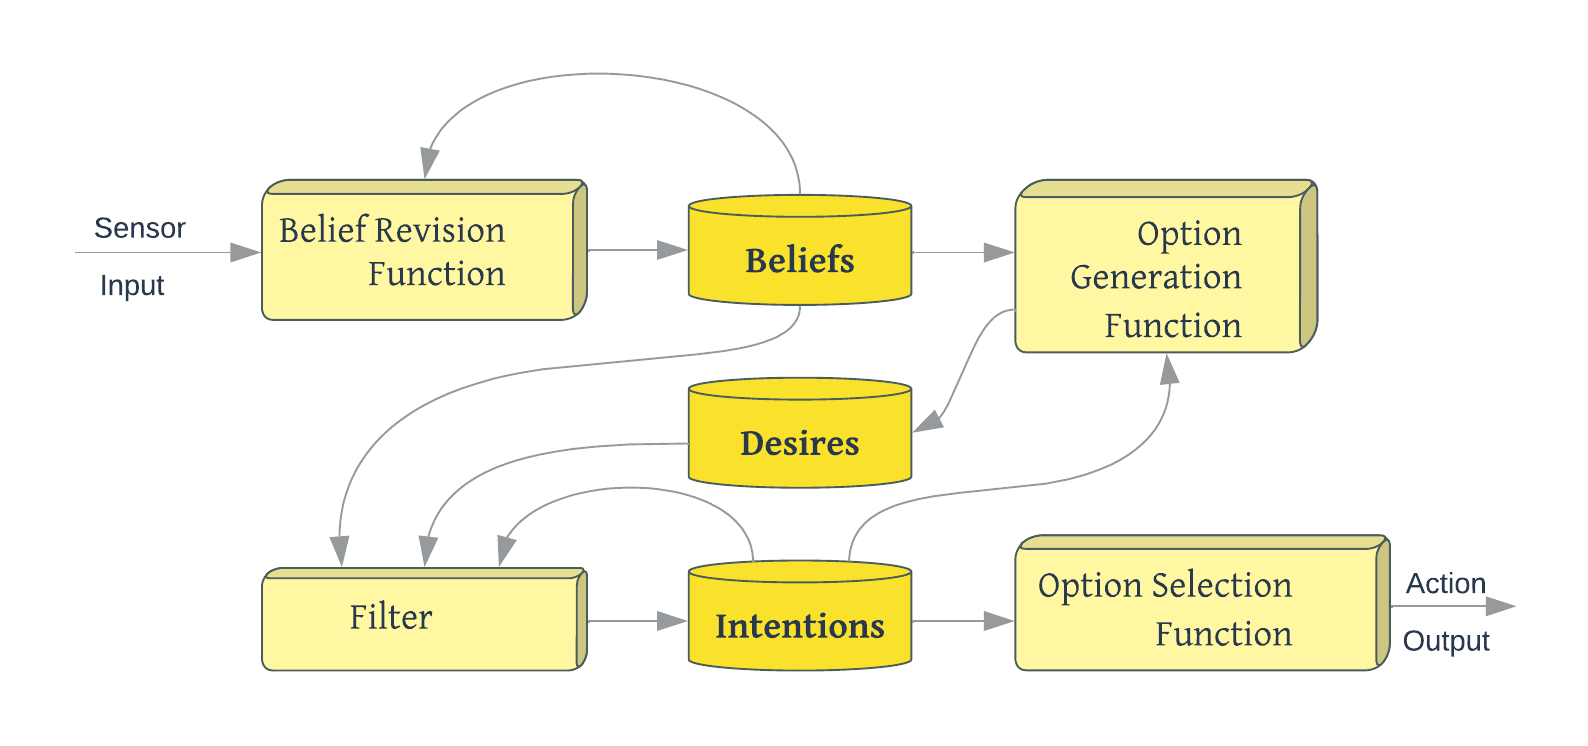
\includegraphics[width=12cm]{includes/figures/BDI_arch.png}
      \caption{\ac{BDI} Architecture}
      \label{BDI Architecture}
    \end{figure}
    
\begin{itemize}
    \descitem{Beliefs} 
    Beliefs reflect the agent's informational state, or its perspective (including itself and other agents). Inference rules can also be included in beliefs, allowing forward chaining to lead to new beliefs. Using the word belief rather than knowledge acknowledges that what an agent believes may or may not be accurate (and in fact may change in the future). One or more belief states and a belief set constitute a belief model.
 
 \vspace{.5cm}
 
    \begin{itemize}[label={}]
        \descitem{Belief set}
        A collection of object diagrams that outline the subject matter of an agent class's beliefs serve as the specification for the belief set. A set of instance diagrams that specify a specific instance of the belief set is referred to as a belief state. Although this is an operational decision, beliefs are maintained in a database (also known as a belief foundation or a belief set).
    \end{itemize}
    
    \vspace{.5cm}
    
    \descitem{Desires}
    Desires indicate the agent's motivational state. They reflect goals or scenarios that the agent wishes to achieve or create.
    
    \vspace{.5cm}
    
    \begin{itemize}[label={}]
        \descitem{Goals}
        A desire that has been embraced for active pursuit by the agent is referred to as a goal. The additional requirement that the collection of active wants must be consistent is added when the term "goals" is used.
    \end{itemize}
    
    \vspace{.5cm}
    
    \descitem{Intentions}
    Intentions depict the agent's deliberate state, or what the agent has decided to do. Intentions are aspirations that the agent has made some commitment to. This indicates that the agent has started carrying out a strategy in implemented systems.
    
    \vspace{.5cm}
    
    \begin{itemize}[label={}]
        \descitem{Plans}
        Plans are collection of instructions that an agent can follow to carry out one or more of its objectives. They can be thought of as recipes or knowledge bases. Plans could incorporate different plans. Three different categories of nodes—start states, end states, and internal states—as well as one kind of directed nape of the neck the plan graph's constituent parts.
        
        \vspace{.5cm}
        
        \begin{itemize}[label={}]
        \descitem{Plan Execution}
        An \textit{activation event} and \textit{activation condition}, which specify when and in what context the plan should be activated, are labeled on the plan graph's first transition. The activation event could be a goal event that happens as a result of the accomplishment of a sub goal activity in another plan, leading to goal-driven activation, or a belief event that happens when an agent's beliefs change or when certain external changes are noticed. If more than one plan is relevant to an event in a particular context, they are either engaged concurrently if the activation is event-driven or progressively until they are successfully terminated if the activation is goal-driven. When a plan is activated, an action may be conducted with the help of an optional activation action.
        
        \vspace{.5cm}
        
        Events pass and fail may be used to indicate the success or failure of the activity connected with the active state during transitions between them. Activities may be halted by transitions from active states that are denoted with the event any whenever their condition is satisfied. The transition of a plan that is aborted is a specific instance of this. The plan fails if the abort condition is true at any point during the execution of its body after it has been triggered. The final transitions of the plan graph may be labeled with the steps to be taken in the event that the plan is successful, unsuccessful, or abandoned.
        
        \vspace{.5cm}
        
        \descitem{Failure}
        The semantics of plan graphs includes the idea of failure. When an action on a transition fails, when there is an explicit transition to a fail state, or when the activity of an active state ends in failure with no outbound transition enabled, failure inside a graph can happen.
        \end{itemize}
    \end{itemize}
    
    \vspace{.5cm}
    
    \descitem{Events}
    In a nutshell, events function as triggers for the agent to react. An event may alter aims, activate plans, or update beliefs. Externally produced events may be picked up by sensors or other connected systems. Events may also be produced internally to start decoupling updates or activity plans.
\end{itemize}

In order to include obligations, norms, and commitments of agents acting within a social context, the \ac{BDI} was further enhanced with an obligations component, giving rise to the \ac{BOID} \cite{boid} agent architecture.


\section{Agent Programming}

In the \ac{AOP} paradigm, the idea of software agents serves as the foundation for the development of the software. \ac{AOP} has externally stated agents (with interfaces and messaging capabilities) at its core as opposed to \ac{OOP}, which has objects (offering methods with variable parameters) at its foundation. They might be viewed as abstractions of actual items. Messages are interpreted in a class-specific manner by receiving "agents."

\subsection{\ac{AOP} versus \ac{OOP}}

\ac{AOP} specialising the framework by fixing the state (now called mental state) of the modules (now called agents) to consist of components such as beliefs (along with beliefs about the world, about themselves, and about one another), capabilities, and decisions, each of which enjoys a precisely defined set of properties. OOP proposes viewing a computational system as being composed of modules that are able to communicate with one another and that have individual ways of handling incoming messages.  Table \ref{AOP versus OOP} summarizes the relation between \ac{AOP} and \ac{OOP}.

\vspace{.5cm}

A variety of restrictions are imposed on an agent's mental state, which generally match to restrictions placed on their common sense equivalents. These agents notify, request, offer, accept, reject, compete, and help one another to do a computation. This concept is directly adapted from the literature on speech acts \cite{speech}. Speech is categorized according to speech acts, which include informing, requesting, offering, and more. Each of these communication acts has a unique set of assumptions and outcomes. \ac{AI}, natural language processing, and plan recognition all use speech act theory.
 Table \ref{AOP versus OOP} summarizes the relation between AOP and OOP

\vspace{.5cm}

\begin{table}[h]
\small
\centering
\caption{\ac{AOP} versus \ac{OOP}}
\label{AOP versus OOP}
\resizebox{11cm}{!}{%
\begin{tabular}{|l| l| l|}
\hline
\textbf{} & \textbf{\ac{AOP} } & \textbf{\ac{OOP}} \\ 
\hline\hline
\textbf{Fundamental Unit} & Agent  &  Object\\ \hline 
\textbf{Parameters defining} & beliefs, commitments,  & Unconstrained\\
\textbf{state of basic unit} &  capabilities, choices .... & \\ \hline 
\textbf{Computation process} & message passing and  &  message passing and \\ 
 & response methods & response methods\\ \hline 
\textbf{Types of message} & inform, request, offer,  & Unconstrained\\ 
 & promise, decline .... & \\ \hline 
\textbf{Constraints on methods} & honesty, consistency ....  &  None\\ 
\hline \hline 
\end{tabular}}
\end{table}

\vspace{.5cm}

\subsection{AgentSpeak(L): \ac{BDI} Agents Interaction}

AgentSpeak(L) is a simplified textual version of \ac{PRS} \cite{prs} or \ac{dMARS} \cite{dmars}. In most ways, the language and its operational semantics are comparable to the implemented system. The implemented system includes extra language constructs to facilitate agent programming.

\vspace{.5cm}

AgentSpeak(L) is a programming language that uses a restricted first-order language with events and actions as its core. The programs created in AgentSpeak(L) govern the agent's behavior (i.e., its interaction with the environment). The agent's beliefs, desires, and intentions are not explicitly stated as modal formulae.

\vspace{.5cm}

The agent's existing belief state may be considered as a model of itself, its environment, and other agents; states that the agent intends to bring about based on external or internal stimuli can be considered as desires; and the adoption of programs to meet such stimuli can be characterized as intentions. This shift in perspective of using a basic specification language as an agent's execution model and then ascribing mental attitudes such as beliefs, desires, and intentions from an external standpoint is more likely to integrate practice and theory.

\subsubsection{Jason}

The agent program and an agent architecture can be differentiate as, the software framework in which an agent program operates is referred to as the agent architecture. The \ac{PRS} is an example of an agent architecture, and the plans are the software that exists within it. We design the program that will drive the agent's behavior, but the architecture itself determines most of what the agent does without the programmer having to worry about it. Jason's language is an extension of AgentSpeak, which is based on the \ac{BDI} architecture. As a result, a belief basis is one of the components of the agent architecture. Another key component is the agent's goals, which are realized through plan execution.

\vspace{.5cm}

It has become customary to include a simple example program to aid comprehension. Hence, an example of Jason AgentSpeak code:

\vspace{.5cm}

\begin{lstlisting}[backgroundcolor = \color{white}, frame=none, numbers=none]
	 started.

    +started <- .print("Hello, I'm an Agent").
\end{lstlisting}

\vspace{.5cm}

Let us attempt to grasp some of what is going on here. The first thing to realize is that this is the definition of a single agent. This specification is generally kept in a single file with the \texttt{'.asl'} extension. Agent's basic beliefs is described in the first line. The full stop, \texttt{'.'}, serves as a syntactic separator in the same way as a semicolon does in Java or C. The next line establishes a plan for the agent, which is the sole plan this agent possesses. This action will display \texttt{'Hello, I'm an Agent'} on the user's terminal. Later, more goals and sub-goals also can be added, according to the plans and requirements.

\subsubsection{Astra}

Astra is also based on AgentSpeak(L) in that it provides all of the same fundamental capabilities as AgentSpeak(L), but it also adds a number of extra features that makes it more practical Agent Programming Language. The fundamental distinction between beliefs, aims, and events is that words and variables are typed. Astra's type system is based on the Java type system, mainly because Java is the underlying implementation language, and using a comparable type system makes translating between Astra and Java easier and more visible.

\vspace{.5cm}
As a result, ASTRA programs are more organized than AgentSpeak(L) applications. The basic structure is seen below:

\vspace{.5cm}

\begin{lstlisting}[backgroundcolor = \color{white}, frame=none, numbers=none]
     package path.to.folder;
     import java.lang.Object;
     
     agent Hello {
         module Console console;
    
         initial !init();
    
         rule +!init() {
             console.println("Hello, I'm an Agent");
         }
     }
\end{lstlisting}

\vspace{.5cm}

As can be observed, Astra has embraced the Java \texttt{package} and \texttt{import} nomenclature. The \texttt{agent} keyword denotes the beginning of the agent program, and curly braces represent the body of that program (known here as an \texttt{agent class}). This specification is generally kept in a single file with the \texttt{'.astra'} extension. This action will also display \texttt{'Hello, I'm an Agent'} on the user's console.

\section{Web3}

\subsection{Background}
The terms "Web 1.0" and "Web 2.0" refer to phases in the development of the World Wide Web using different technology and formats. Web 1.0 refers to a time when the bulk of websites just had static pages and the great majority of people consumed information rather than created it. Web 2.0 is centered on user-generated content that is published to forums, social media and networking sites, blogs, and wikis, among other services. It is founded on the concept of "the web as platform."

\subsection{Introduction}
An notion for a new version of the World Wide Web called Web3 (sometimes referred to as Web 3.0) integrates ideas including decentralization, blockchain technology, and token-based economy. Some journalists and engineers have compared it to Web 2.0, where they claim that content and data are concentrated in a select few businesses frequently referred to as "Big Tech."

\vspace{.5cm}

Web3's specific goals vary, and the phrase has been characterized as "ambiguous," but they all revolve on the concept of decentralization and frequently include \ac{BCT}, including multiple crypto-currencies and \ac{NFT}. The concept of Web3 would include financial resources, in the form of tokens. It can alternatively be described as the ostensible next generation of the web's technological, legal, and monetary infrastructure, which includes crypto-currencies, blockchain, and smart contracts. Web3's three core architectural enablers were recognized as a mix of decentralized or federated platforms, safe interoperability, and verifiable computing via distributed ledger technologies.

\vspace{.5cm}

The idea of \ac{DAO} serves as the foundation for several concepts. On addition to owning your data in Web3, you can also use tokens that function like stock to collectively own the platform. \ac{DAO} enables decentralized platform ownership coordination and future platform decision-making. Another important idea is \ac{DeFi}, which allows for money exchange without the intervention of banks or the government. \ac{SSI} enables users to identify themselves without depending on an authentication system like OAuth \cite{oauth}, where identity verification requires contacting a trusted party. Web3 would most likely coexist with Web 2.0 websites, with Web 2.0 websites most likely adopting Web3 technology to keep their services updated.

\subsection{Concept}

Web 3.0 may be recognized by a collection of traits that are altering how people connect outside of the physical world and have an impact on how businesses are made: 
\begin{itemize}

    \item  Individualized - Information may be divided into context-relevant segments based on network contacts and personal preferences. In fact, one of the features of Web 3.0 is the capacity to deal with unstructured content on the Web more intelligently by giving the published data about individual or group factors contextual meaning. The social networks are a well-known method of connection with a very broad audience of adopters. People may choose their own exposure and contacts depending on information preferences and "proximity".

    \item 
  Ubiquity - People can connect at any time and from any location. Staying connected is made easier by a variety of communication alternatives, including mobile networks, Wi-Fi networks, cable networks, or cellular networks, as well as many device kinds, including laptops, desktop computers, tablets, and an endless array of mobile devices. Regardless of the architectures or systems being used


    \item  Efficient - Both people and computing devices are capable of filtering information based on context, meaning, and relevance. This trait has an implied connection to the individualized trait. Regarding individual variances, knowledge causes various responses in various persons. The capacity to filter content based on user interests appears to be a benefit of Web 3.0. Efficiency requires that the information must be organized such that algorithms can read it and comprehend it as clearly and completely as humans can.

\end{itemize}
\section{Blockchain}

\subsection{Introduction}
Blockchain is a decentralized ledger system that may be used to store data across numerous cluster nodes. A typical blockchain network's cluster of nodes cannot be controlled by a single organization, hence the system is decentralized. The blockchain data is computationally authenticated by the majority of unconnected nodes in a cluster of arbitrary 'N' nodes. This fundamental architecture of blockchain assures that it is not controlled by a centralized authority and that the system as a whole is 'trustless.' We imply that there is no need to trust the source of data or the provider since mathematical computations and decentralized validation make the system computationally trustworthy.

\vspace{.5cm}

Due to the lack of a single administrator who has access to change and remove the recorded data, this feature of blockchain technology assures that the data has not been altered. It displays characteristics like immutability, irrevocability, and non-repudiation as a result of its construction. Due to these characteristics, it is the perfect answer for several significant real-world use cases, including financial applications.

\vspace{.5cm}

The modern blockchains allow users to create their own custom code that is then performed as functions inside the ecosystem and the outputs of these functions are added to the blockchain's updated state. These functions are often run at numerous network nodes and a consensus on the status of outcomes is reached. These tasks or workloads are known as smart contracts in Ethereum and several other public blockchains, and chaincodes in Hyperledger Fabric.


\subsection{Architecture}
According to its technical definition, a blockchain is a series of interconnected blocks that, as seen in Figure \ref{Blocks chained together in a blockchain}, include the data on a group of transactions up to the most recent block. The block headers retain the details of their own hash, that of their preceding block, a list of transactions, and the time stamp. In the blockchain network, these characteristics are utilized to track a specific transaction. All blockchain nodes save a block as the most recent state once it has been approved and confirmed by the majority of network participants.

 \vspace{.5cm}
 
\begin{figure}[h]
  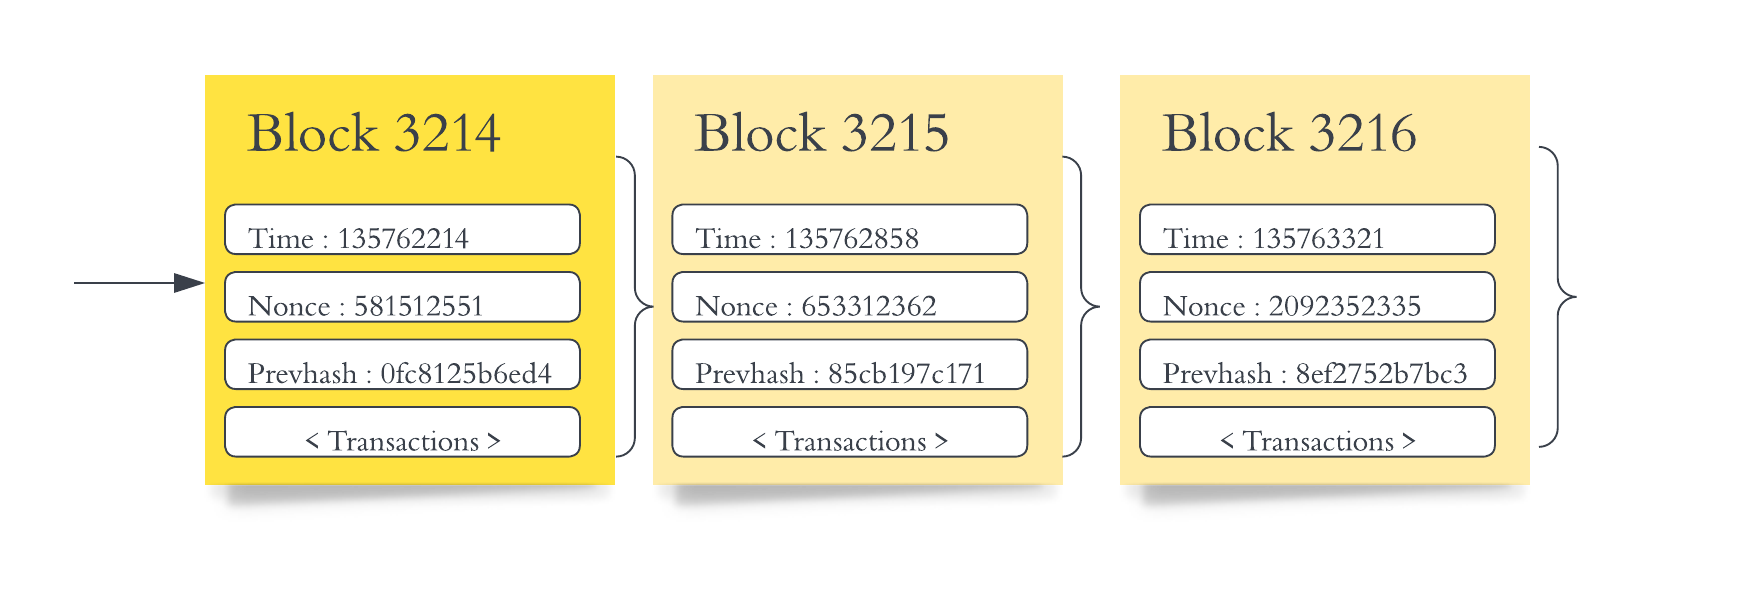
\includegraphics[width=\textwidth]{includes/figures/blocks.png}
  \caption{Blocks chained together in a blockchain}
  \label{Blocks chained together in a blockchain}
\end{figure}

 \vspace{.5cm}
 
Different procedures, including as \ac{PoW} \cite{pow}, \ac{PoS} \cite{pos}, and \ac{PoA} \cite{poa}, etc., are available to reach agreement on the choice of a block.
 
\vspace{.5cm}
 
On a higher level, blockchains may be split into two categories: permissioned and permissionless. Consortial and private blockchains are also included in the permissioned blockchains, whereas public blockchains are included in the permissionless blockchains. Below, we explore these categories' characteristics.

\subsubsection{Public Blockchains}

Public blockchains are permission-less blockchains in which anybody with a personal computer may run an open-source protocol and connect to the network as an equal node. The public blockchains run completely decentralized peer-to-peer systems. They are the perfect approach for implementing digital currency. The most well-known public blockchains are Ethereum and Bitcoin.

\subsubsection{Private Blockchains}

Private blockchains are distributed node clusters that operate within a secure private network and store and process data according to blockchain rules. Private blockchains are governed by a centralized organization rather than being decentralized in nature. They primarily serve as a distributed ledger that is scalable. Private blockchains often employ the lightweight \ac{PoA} protocol to add new blocks.

\subsubsection{Consortial Blockchains}

Consortial blockchains are permissioned blockchains, just as private blockchains, and the general public cannot join them. They belong to a group of priveleged individuals who could be associated with this network. The cluster of nodes is dispersed throughout the intranets of the participating organizations. They are especially helpful when two mutually trusted parties wish to use the distributed ledger's privacy-preserving features. Hyperledger Fabric, Hyperledger Indy, and other consortium blockchains are the most well-known.


\subsection{Smart Contracts}

To begin, we will define smart contracts. Szabo's \cite{def1} definition is as follows:

\vspace{.5cm}

\begin{definition}
  A smart contract is a set of promises, specified in a digital form, including protocols within which the parties perform on these promises.
\end{definition}

\vspace{.5cm}

In order to automatically execute, control, or document legally significant events and activities in accordance with the provisions of a contract or an agreement, a smart contract is a computer program or transaction protocol. The goals of smart contracts are to decrease the need for trustworthy intermediaries, arbitration fees, fraud losses, and malicious and unintentional exceptions. The smart contracts provided by Ethereum are widely regarded as a crucial building block for \ac{DeFi} and \ac{NFT} applications. Smart contracts are frequently linked to cryptocurrencies.

\vspace{.5cm}

A smart legal contract, as opposed to a smart contract, is a conventional, legally-binding pact with specific provisions defined and put into machine-readable code. Smart legal contracts should not be confused with smart contracts.

\subsection{\ac{EVM}}

The second-largest blockchain system in the world is believed to be Ethereum. With smart contracts, Ethereum enhances the blockchain paradigm. The applications running on the Ethereum blockchain are known as smart contracts. Ethereum provides the \ac{EVM} to parse the source code of the contracts into an opcode sequence that is predefined by Ethereum in order to execute the smart contracts. For the Ethereum blockchain to correctly execute contracts and handle transactions, each node requires an \ac{EVM}.

\vspace{.5cm}

The \ac{EVM} may be conceptualized practically as a vast, decentralized system with large numbers of objects, called \textit{accounts}, that can maintain an internal database, run code, and communicate with one another.

\subsection{Solidity: Build Smart Contracts}

The Ethereum blockchain's popularity and disruptive power are directly related to its capacity to execute smart contracts. \ac{BCT} may be effectively used to create \ac{Dapp} using Ethereum platform. A \ac{Dapp} is a tool used to connect individuals and groups on various sides of an interaction without the usage of a centralized intermediary.

\vspace{.5cm}

\textit{Solidity}, a Javascript-like language designed expressly for creating smart contracts, is the primary language used in Ethereum. Among its other characteristics, Solidity is statically typed and enables complicated user-defined types, libraries, and inheritance. The solidity compiler converts source code into \ac{EVM} bytecode so that it may be deployed into the Ethereum network. The owner of the contract is responsible for paying the additional transaction fees associated with contract deployments and smart contract interactions in the form of \textit{gas}.

\subsection{Truffle Suite}
\subsubsection{Truffle}

As a programming environment, testing framework, and asset pipeline for blockchains running on the \ac{EVM}, truffle basically aims to simplify the workload of a developer. Truffle offers built-in binary management, deployment, linking, compilation, and testing for smart contracts in addition to automated contract testing for quick development. It offers configurable build pipeline with support for tight integration, as well as pNPM ackage management using \ac{NPM} and the ERC190 standard, i.e. \ac{ERC}.

\vspace{.5cm}

Truffle supports transactions and deployments with MetaMask to safeguard your mnemonic, which is a pattern of letters, and it offers enhanced debugging with breakpoints, variable analysis, and step functionality.
With an interactive terminal for direct contract communication, it is an external script runner that runs scripts inside the Truffle environment.
Provides a scriptable, extendable framework for deployment and migrations, as well as network management for deploying to any number of public and private networks.

\subsubsection{Ganache}

Ganache is a private blockchain enabling speedy production of Corda and Ethereum distributed applications. Ganache may be used throughout the whole development cycle, allowing you to create, distribute, and test \ac{Dapp} in a secure and predictable setting.

\vspace{.5cm}

Both a \ac{UI} and a \ac{CLI} are available with ganache. A desktop program called Ganache \ac{UI} supports both Corda and Ethereum. Ethereum programming is possible using the powerful command-line tool ganache. It supports snapshot/revert state, Ethereum JSON-RPC compatibility, Zero-config Mainnet and testnet forking, console-log in Solidity, and the ability to impersonate any account without the need for private keys.

\subsection{Vision}
As blockchain technology continues to develop, a number of new blockchains have recently come to light, each with a unique architecture and implementation that has been carefully chosen for the intended use case. Additionally, there are significant flaws in the conventional blockchain architecture that remain unresolved, and other implementations aim to address these concerns. (1) Lack of anonymity in transaction execution (2) High transactional delay owing to complex consensus procedures that cause scalability concerns are the two main outstanding challenges with blockchains. (3) Communication between several blockchains; (4) Integration with the outside world.

\vspace{.5cm}

Each of the more recent blockchain implementations, including Zcash, Polkadot, Ethereum 2.0, Chainlink, etc., is working to find a solution to these problems. With the use of trustworthy execution environments, we also hope to address the aforementioned issues with conventional blockchains in this thesis. Because the burden from the blockchain is transferred to secure execution environments, the blockchains are lightweight and offer transaction execution privacy. In addition, the Hyperledger Avalon has developed blockchain connectors for a number of distinct blockchains that may be used to promote interoperability between them. The Avalon infrastructure may also be used to build "attested oracles," which connect blockchains with data from the outside world.


	\ifx\doclanguage\english
\chapter{Design}

This chapter describes the layout of the thesis' proposed solution. The \ac{BDI} agents work in a \ac{MAS} via Jason AgentSpeak and communicate via solidity and python-based smart contracts. We would talk about the application's design objectives and general overview. We will also go through the application's design and functionality for both creating smart contracts independently and after doing so, as well as for creating agents. This chapter's prerequisites include understanding the design and architecture of blockchain, AgentSpeak, and \ac{AOP} as described in the previous chapter. The prior chapter's contents should be reviewed in order to fully comprehend the chapters that follow.

\section{Roadmap}
.......

\section{Model Description}

    \begin{figure}[h]
    \centering
      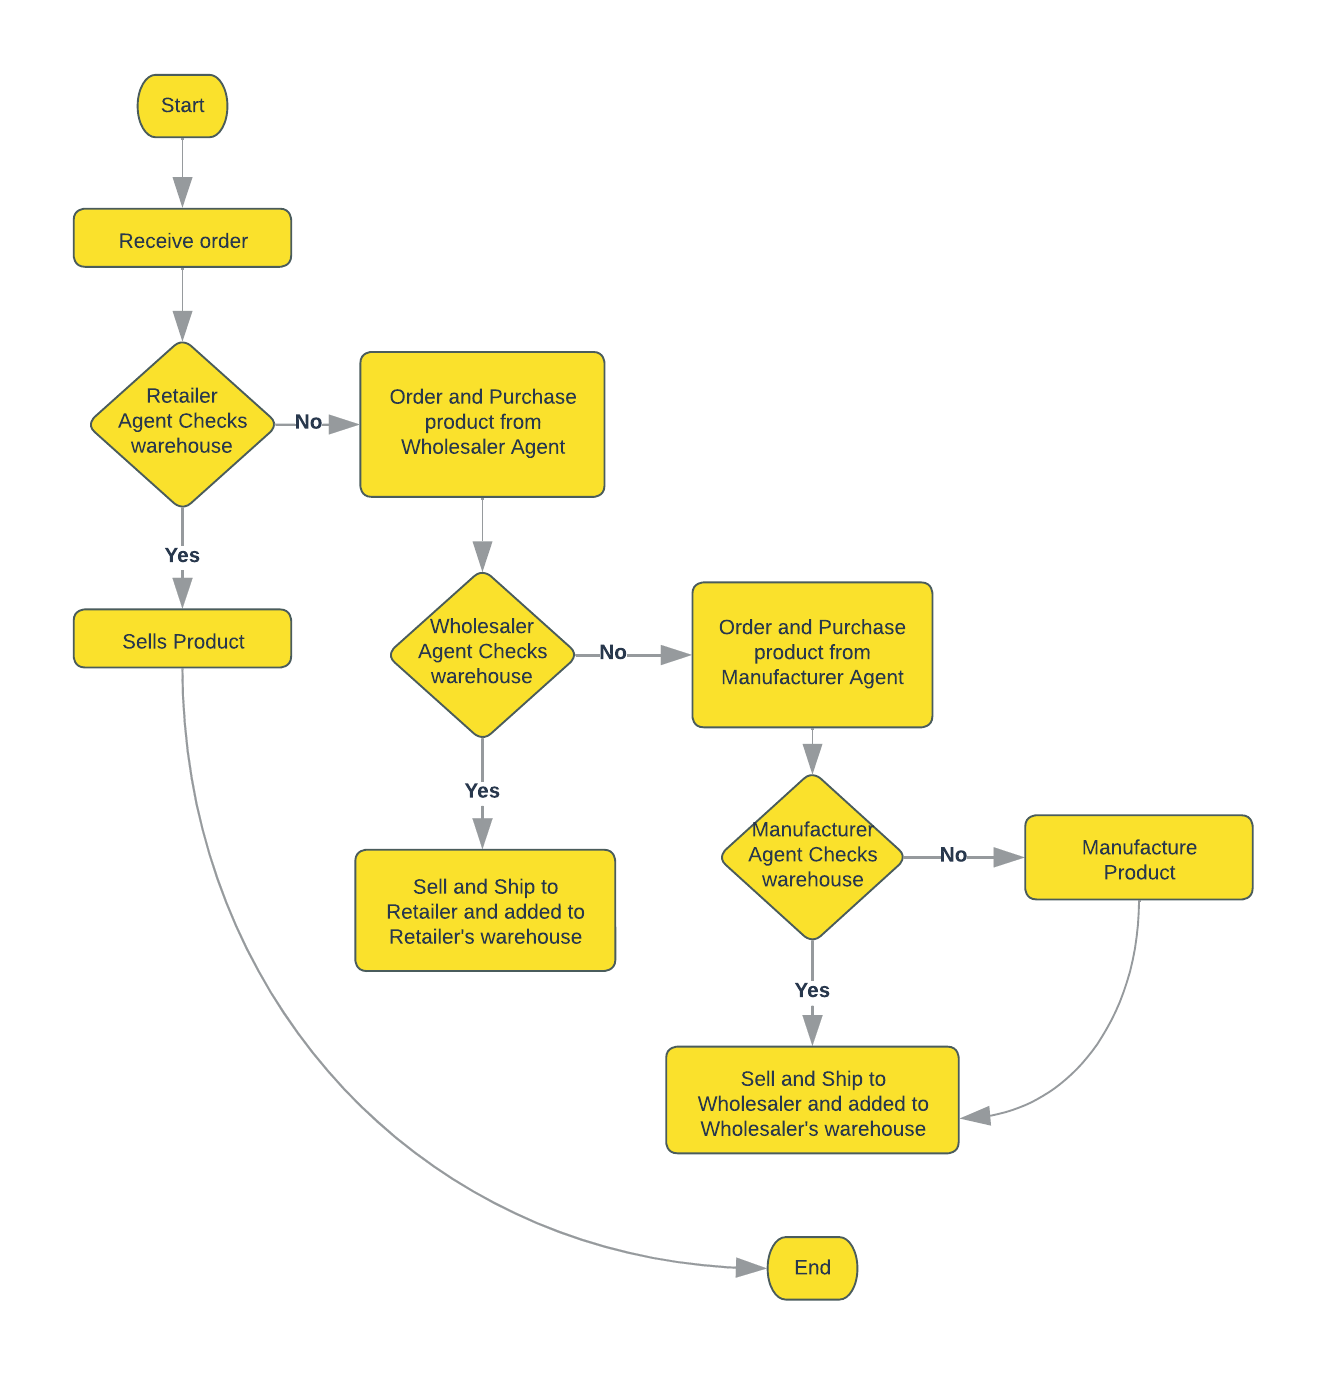
\includegraphics[width=10cm]{includes/figures/Flow Chart.png}
      \caption{Supply Chain Flow Chart}
      \label{Flow chart}
    \end{figure}


The application flow for the \textit{Smart contract development with Jason \ac{BDI} agents} is depicted in Figure  \ref{Flow chart}. These three agents, a manufacturer, a wholesaler, and a retailer, each perform a specific function in the supply chain. All three of the other agents are being invoked by another primary agent in the \ac{MAS}. Figure \ref{Sequence Diagram} may be used to demonstrate this.

   \begin{figure}[h]
    \centering
      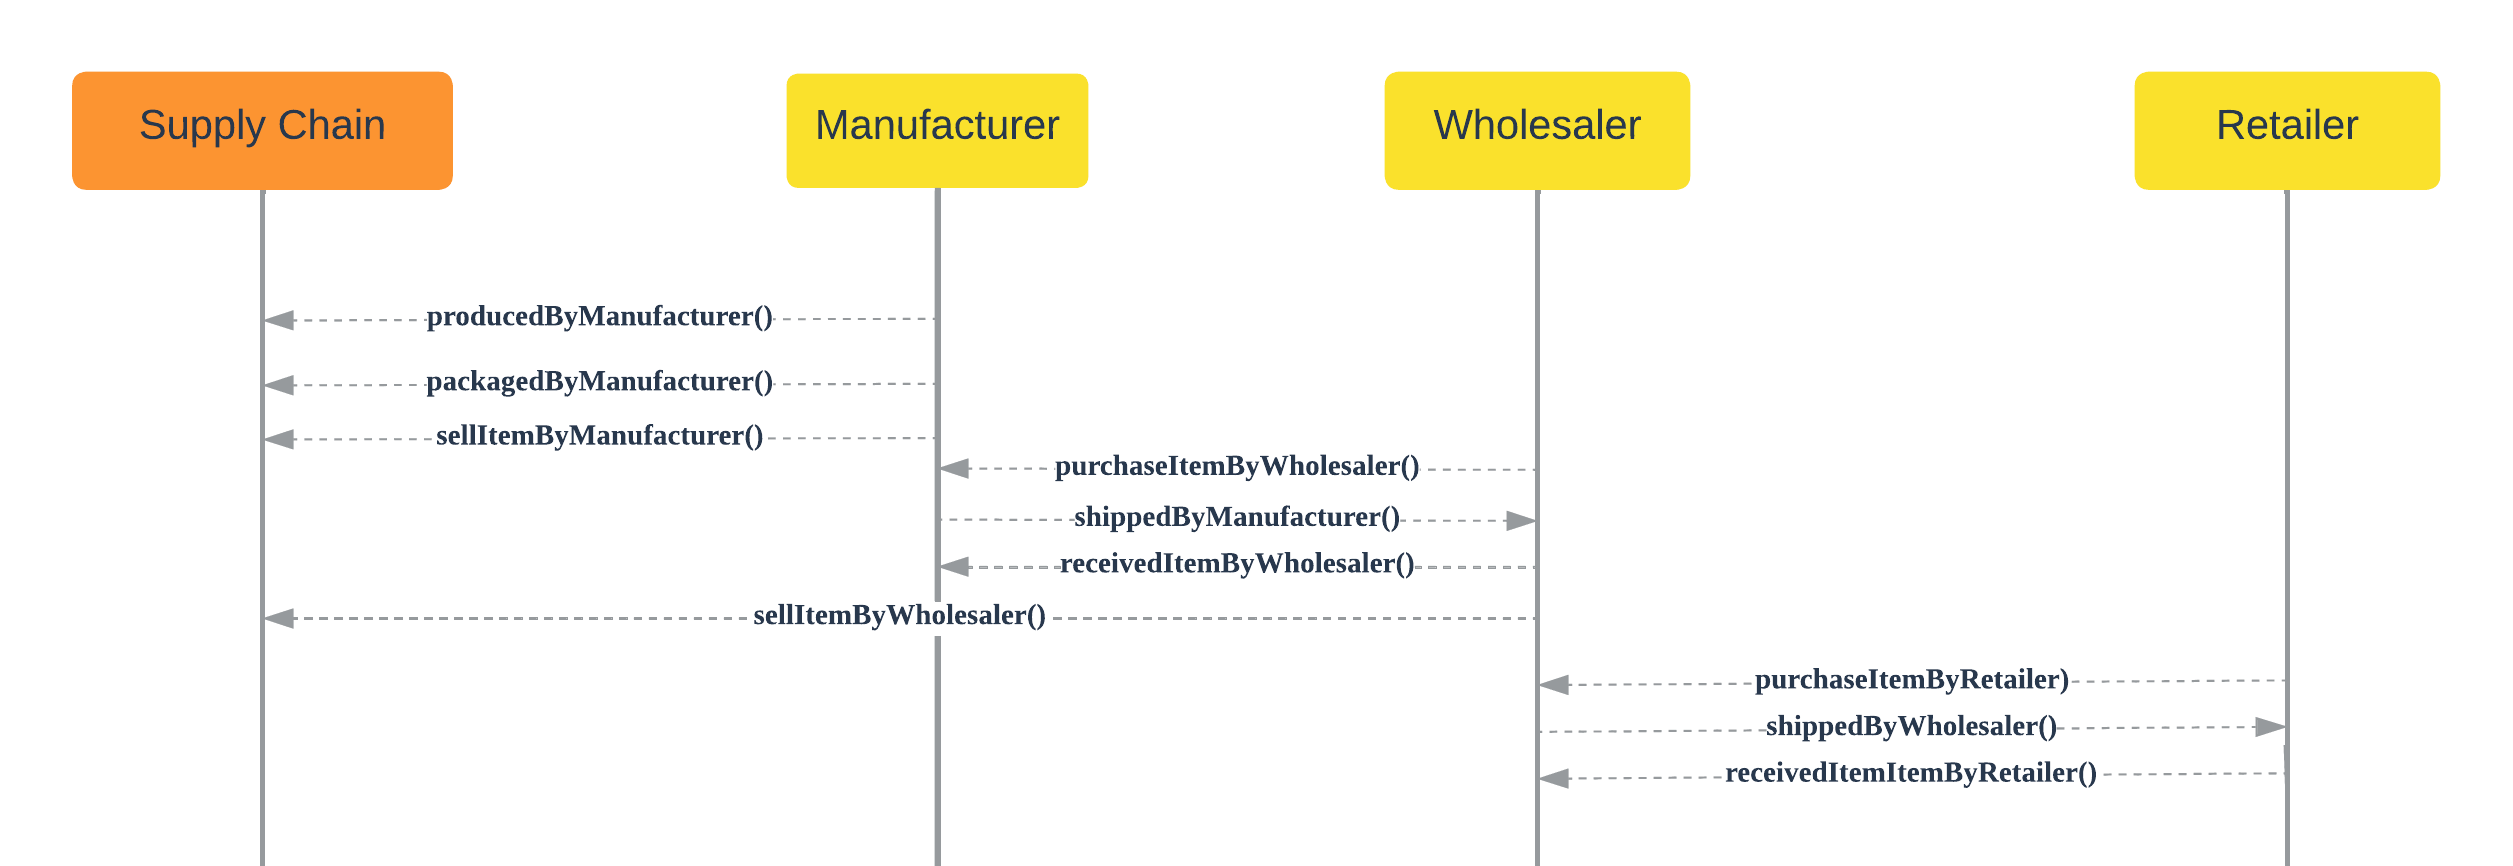
\includegraphics[width=\linewidth]{includes/figures/Sequence diagram.png} 
      \caption{Supply Chain Sequence Diagram}
      \label{Sequence Diagram}
    \end{figure}

\section{Design Goals}

\begin{itemize}

    \descitem{Autonomous}
    To fulfill the objectives assigned to an agent, autonomy simply implies being able to work autonomously. An autonomous agent, thus, at the very least, makes independent judgments about how to accomplish its given goals; these decisions (and subsequently, its actions) are within its own control and are not influenced by other forces.
    
    \descitem{Efficiency}
    Effectiveness strategies improve the functioning of a smart contract or lower the expenses connected with its use. These patterns can help operators and consumers save time and money.
    
    \descitem{Access Control Patterns}
    Particular smart contract functionalities are only accessible by certain people, according to access control rules. For a specific task, permissions and authorizations can be managed, such as limiting access to the admin. On a public blockchain ledger, where everyone can observe the contract but you want to limit who may do what within the contract, the ability to restrict access is especially helpful. Certain access control patterns, such multi-authorization, ownership, and role-based access control, have names that make it obvious what they are meant to do.
    
    \descitem{Goal-directed behaviour}
    If an agent has been assigned a specific objective, it is assumed that the agent would attempt to attain the goal. Proactivity eliminates completely passive actors who never strive to accomplish anything.

    \descitem{Reactiveness}
    Implementing an application that achieves an appropriate mix of goal-directed and reactive behavior becomes difficult. This is one of the primary design goals of AgentSpeak.
    
    \descitem {Security}
    Protection patterns are created to optimize a smart contract's level of security against any threat. Reentrancy attacks, overflow assaults, or the problematic behavior of the actual smart contracts are all prevented by using them. There are various different types of frequently utilized security patterns, which is not surprising given the quantity of assets connected to smart contracts. Numerous of these patterns, such as circuit breakers and evacuation plans, are intended to safeguard contracts against failure in the event that the worst occurs.
\end{itemize}

\section{Contracts Overview}   

While taking into consideration the scenario of a supply chain where all information on suppliers, recipients, products, and business circumstances is dispersed over supply chain databases.
It is possible to execute the sale of products or services as a transaction that is cryptographically signed by the seller and the buyer and attached to a smart contract for sales transactions. When the sale occurs and all other conditions, such as documentation and quality checks, are met, the execution of the transfer of the corresponding funds and rights can be enforced; in other words, smart contracts can ensure that collaborative and entrepreneurial processes are carried out correctly.

\vspace{.5cm}

As aforementioned, the terminology blockchain refers to two things: a distributed database and a data structure (i.e. a linked list of blocks containing transactions, where each block is cryptographically chained to the preceding one by incorporating their hash value and a cryptographic signature, in such a manner that changing an earlier block requires re-creating the whole chain since that block). The idea of smart contracts, which are scripts that run every time a specific kind of transaction takes place and may read and write to the blockchain, is related to the blockchain technology. Smart contracts enable parties to enforce the requirement that while one transaction occurs, other transactions also occur.

    \begin{figure}[h]
    \centering
      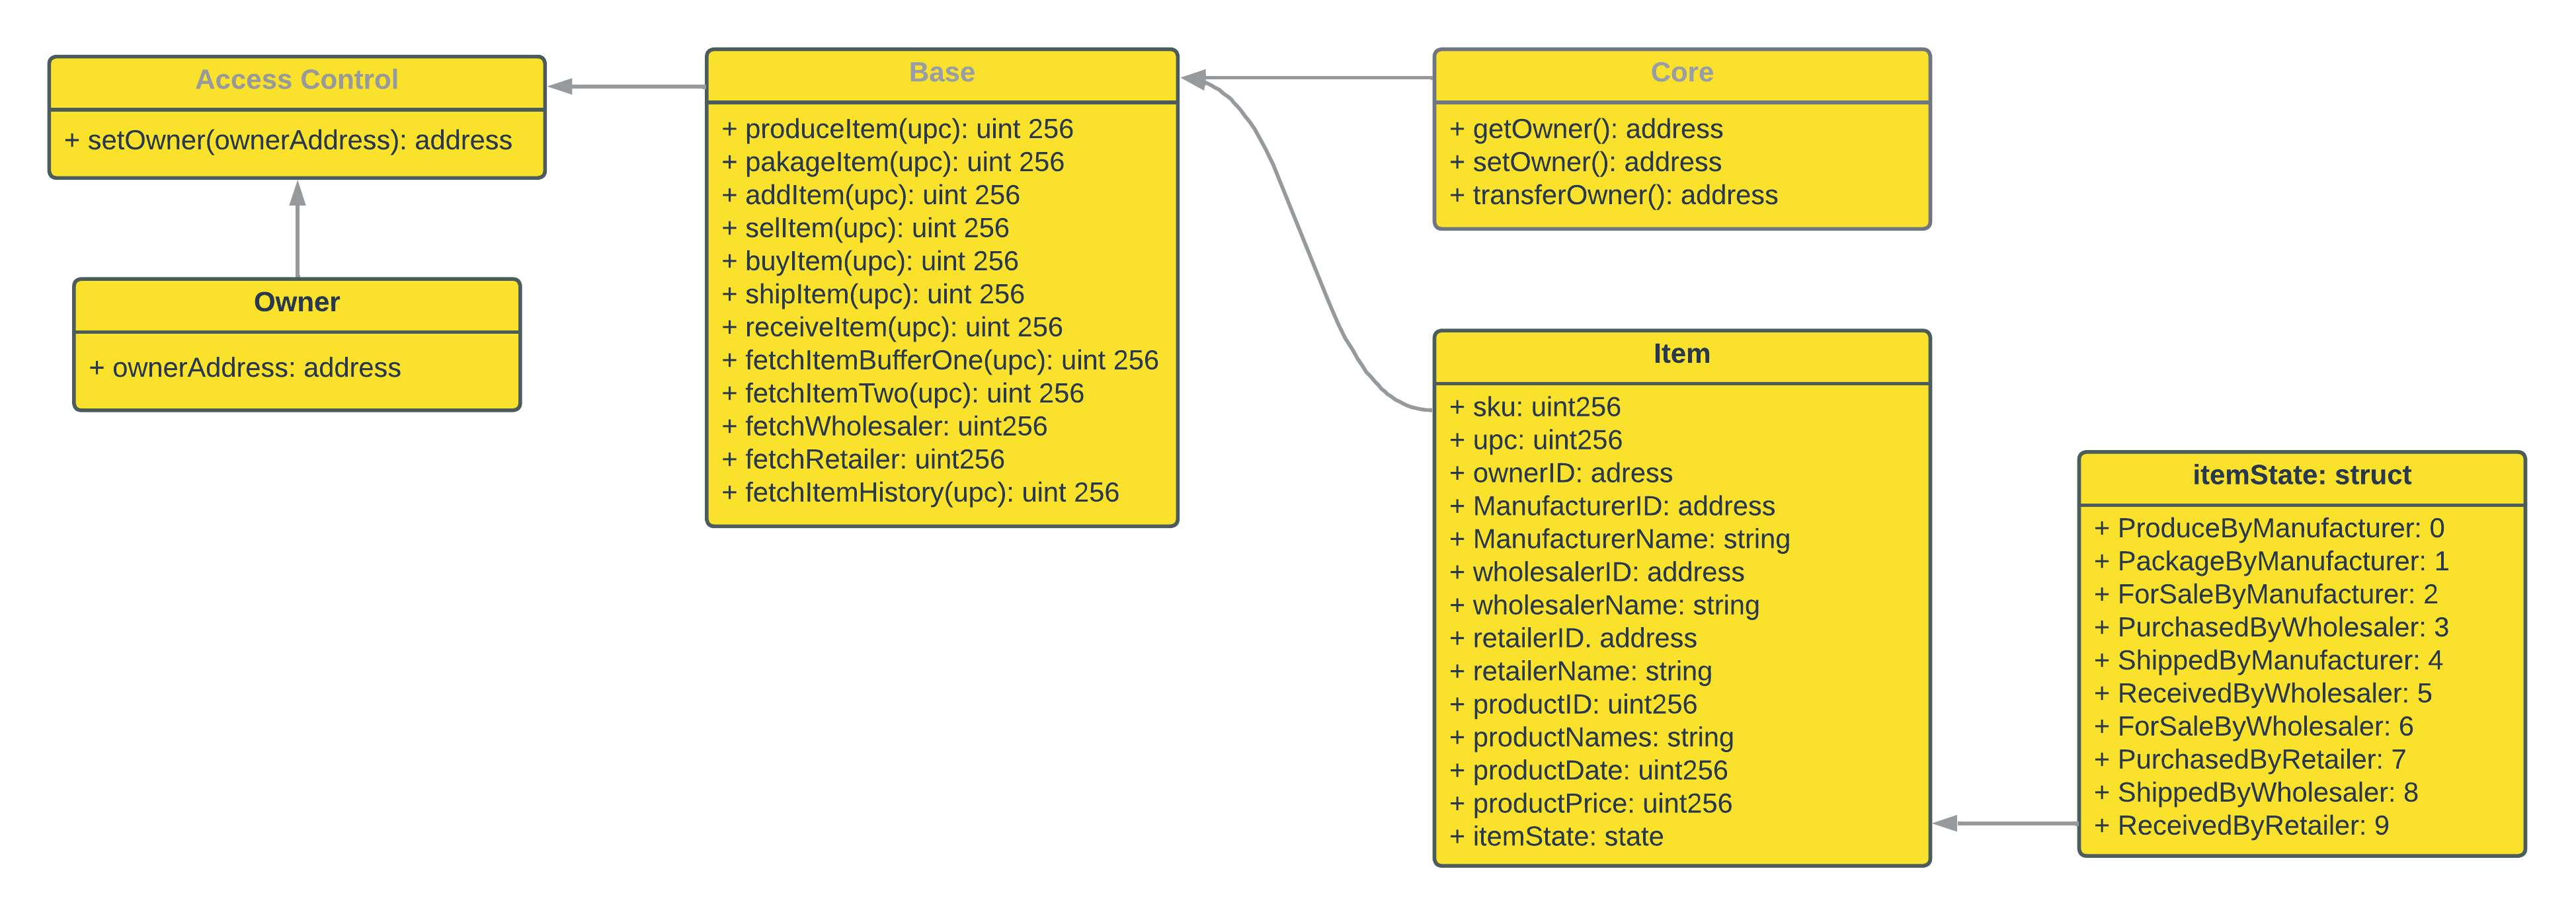
\includegraphics[width=15cm]{includes/figures/Data Model diagram.png} 
      \caption{Data Model Diagram}
      \label{Data Model diagram}
    \end{figure}
    
\vspace{.5cm}

The programming for smart contracts related supply chain is done using Solidity Language while keeping the version in mind in order to integrate it with the agent programming language so that they can work together. Smart contracts perform the following functions: (1) The product is produced by the manufacturer, (2) the manufacturer completes the packaging, (3) the product is placed on the market, (4) the wholesaler purchases the product, (5) the manufacturer ships the product, (6) the wholesaler receives the product, (7) the wholesaler places the product on the market, (8) the retailer purchases the product, (9) the wholesaler ships the product, and (10) the retailer receives the product as the final result.

\vspace{.5cm}

Each function is regarded as an event, and every event is given a state, as shown in Figure \ref{Data Model diagram}. It has always been a rule that each event must occur after the one before it has concluded. For example, a manufacturer cannot sell a product before producing it, while a wholesaler cannot receive a product before buying it. It is carried out with the aid of a state check. A product can also be tracked using the \ac{UPC} or by utilizing the \ac{SKU} to trace the entire batch.

\section{Agent Model}

An agent continually perceives its environment, makes decisions about how to act to achieve its objectives, and then takes action to alter the surroundings. The speech-act theory is commonly used to describe agent communication in \ac{MAS}. The speech-act hypothesis is based on the premise that language is action.

\vspace{.5cm}

\begin{figure}[h]
    \centering
      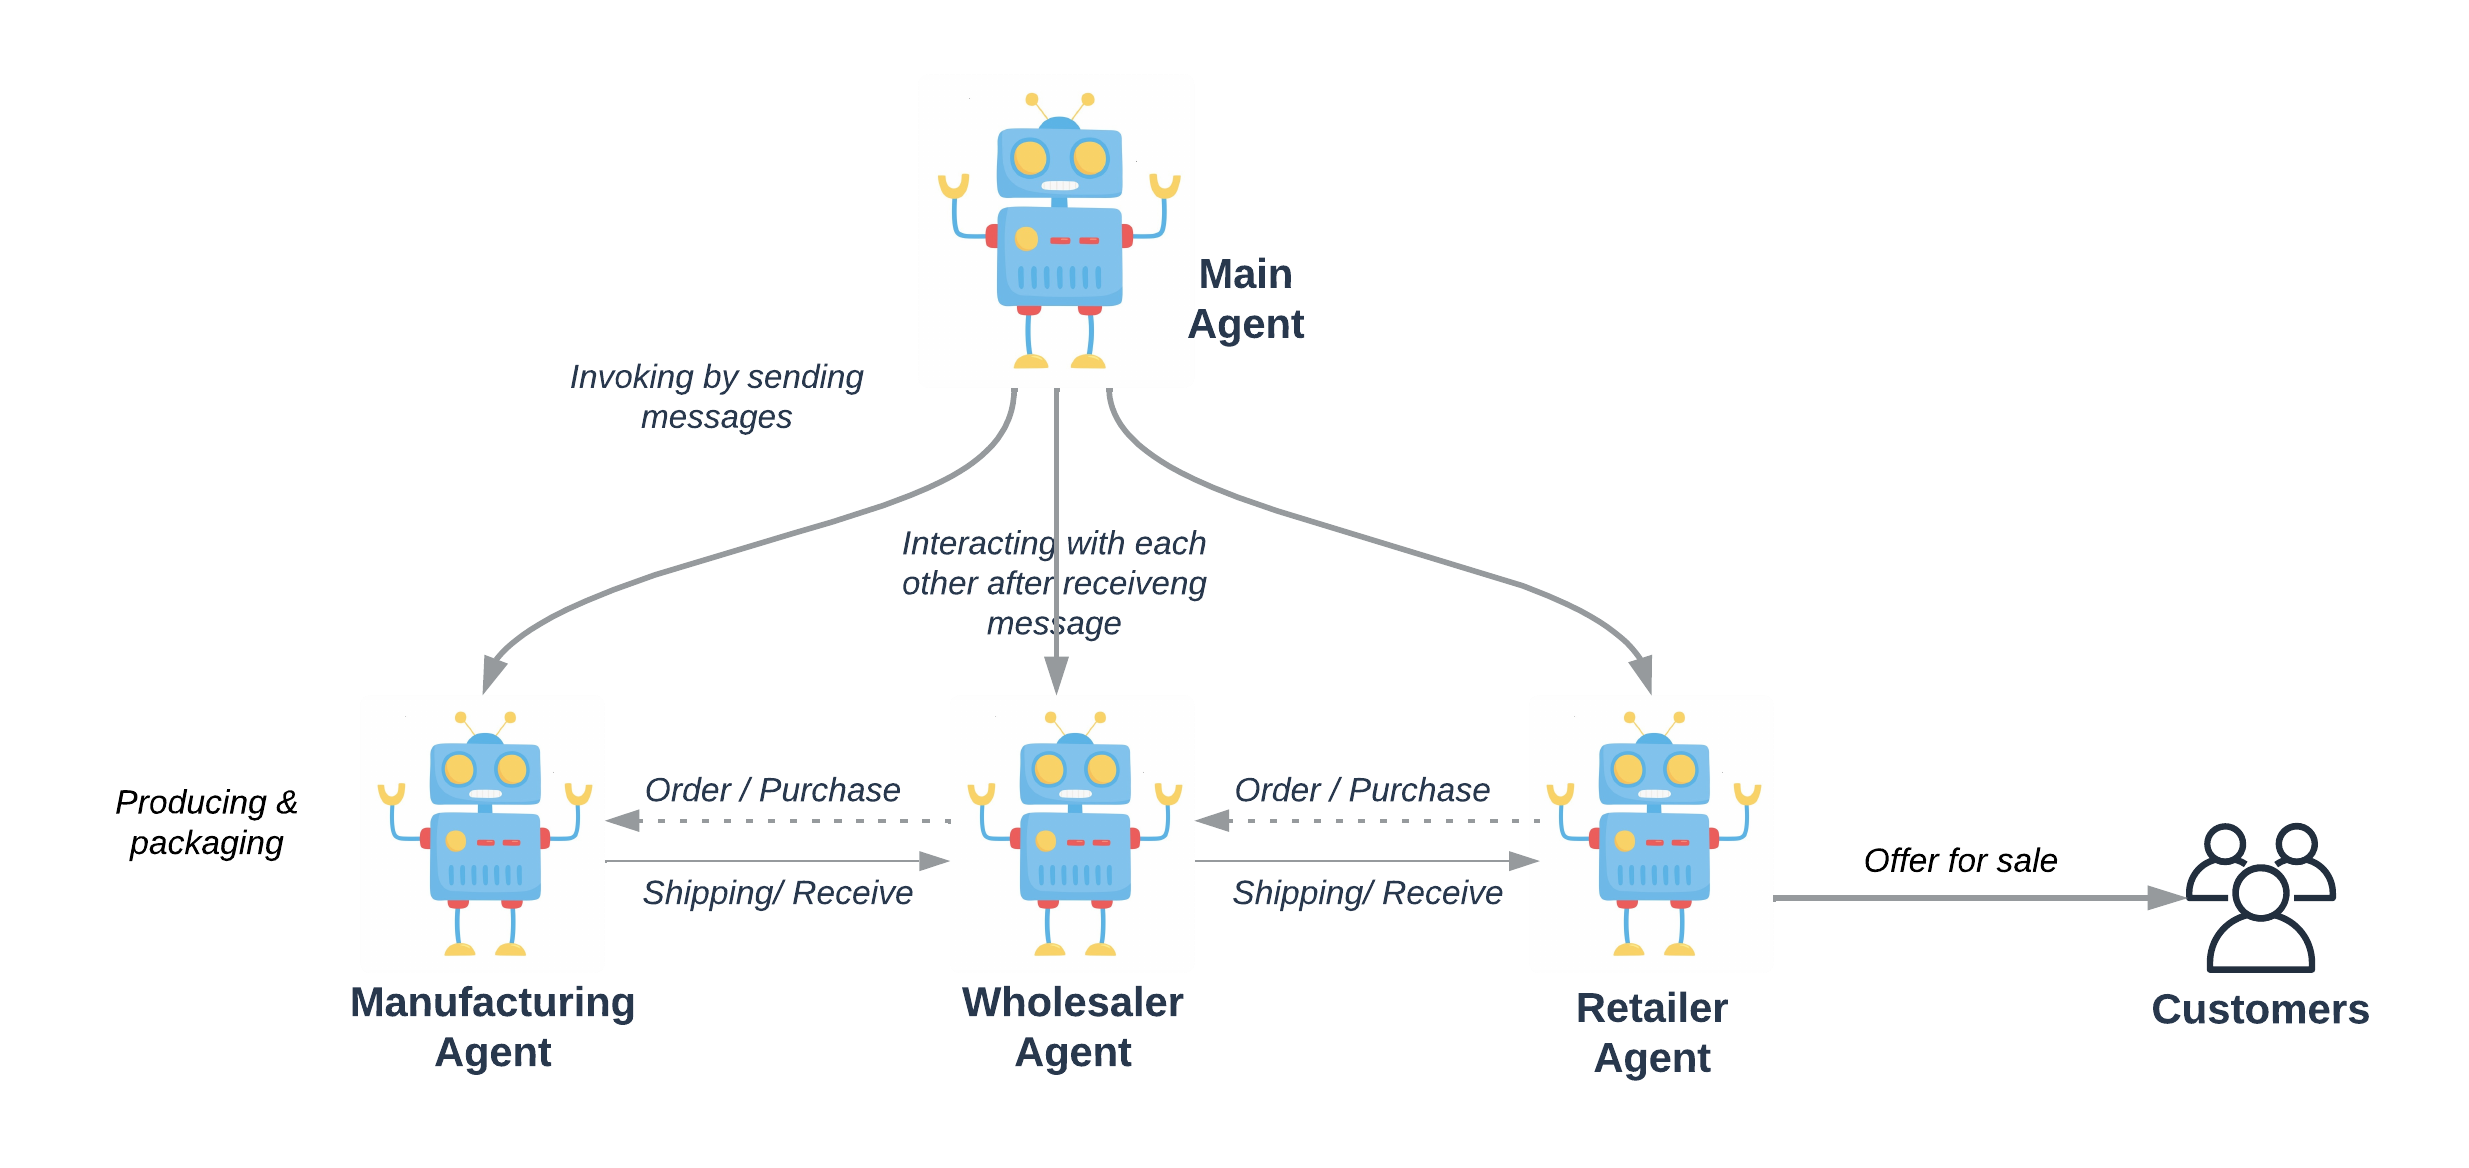
\includegraphics[width=\linewidth]{includes/figures/agent.png} 
      \caption{Agent Interaction in Supply chain}
      \label{Agent Interaction}
    \end{figure}
  

An agent program is run by the Jason interpreter. An agent uses a reasoning cycle to carry out its operations, which may be broken down into the following steps: first, it perceives the environment; second, it updates the belief base; third, it receives communication from other agents; fourth, it selects "socially acceptable" messages; fifth, it chooses an event; sixth, it retrieves all relevant plans; seventh, it determines the applicable plans; eighth, it chooses one applicable plan; and last, it executes one step of an intention.

\vspace{.5cm}

In our \ac{MAS}, each participant's function within the supply chain will be handled by an agent , see figure \ref{Agent Interaction}. The retailer agent will work to ensure that the product is available in the warehouse before ordering it from the wholesaler agent, who will then ask the wholesaler to check its inventory, get in touch with the manufacturer to produce the product, and ship it to the wholesaler, who will then send it to the retailer agent. There will be a \textit{main agent}, who will launch the retailer agent's efforts to sell items to consumers and also other agents by sending messages.
	\chapter{Implementation}

This chapter discusses implementation specifics and the tools used to build smart contracts and jason \ac{BDI} agents. We discuss the \ac{MAS} and \ac{BCT} implementation specifics, package and library versions utilized, and system configuration. Additionally, the procedures necessary to combine both in order to contribute to this thesis are also presented.

\section{System Configuration}

The application was created and tested on a Linux Ubuntu 22.04.1 LTS system.
Visual Studio and InetlliJ are the \ac{IDE}s used to create the application. jEdit is also used somehow to run agents using Jason while creating \texttt{.asl} and running \texttt{.mas2j} file.
To test the compatibility of web3j with gradle for agents, many versions of Java Standard Edition Development Kit were utilized, however the most commonly used was Java SE Development Kit 18.0.2.1. 

\vspace{.5cm}

Other standards for the development of Smart contracts and agents are detailed in the sections below.

\section{Agent Implementation}

The \ac{BDI} architecture is the most common technique to implementing "intelligent" or "rational" agents. The specification of a set of base beliefs and a set of plans results in the creation of an AgentSpeak(L) agent. AgentSpeak(L) differentiates between two kinds of goals: achievement goals and test goals. However, we use achievement targets for our agents. We employed a variety of techniques while writing our agents and ensuring that they could be utilized with smart contracts. We tested several different interpreters and wrote our agents using those. We pursue the following strategies:

\begin{itemize}
    \item \textbf{Jason interpreter built on Java}
    \item \textbf{\ac{ASTRA}}
    \item \textbf{Jason interpreter built on python}
\end{itemize}

The structure of the agent program is governed by the fact that there will be four agents in the MAS, as shown in Figure \ref{Agents in MAS} in MAS, and they will interact with each other as shown in Figure \ref{Agent Interaction}. Our implementation strategy is as follows:

\begin{itemize}
    \item The supply chain will be initiated by the main agent, who will then engage the retailer agent;
    \item Retailer agent will inspect its inventory and sell products to customers; if a product is not in stock, retailer agent will ask the main agent to contact the wholesaler agent;
    \item The wholesaler agent will check its warehouse and ship the product to the retailer agent; if the product is not available, the wholesaler agent will request that the manufacturer agent be contacted by the main agent;
    \item Upon checking its inventory, the manufacturer agent will ship the product to the wholesaler agent. If the product is not in stock, the manufacturer agent will manufacture the product, does the package and deliver it to the wholesaler.
\end{itemize}

Every implementation uses the same approach to how agents cooperate and communicate, and each implementation is detailed in more detail in the section below.

\begin{figure}[h]
\centering
  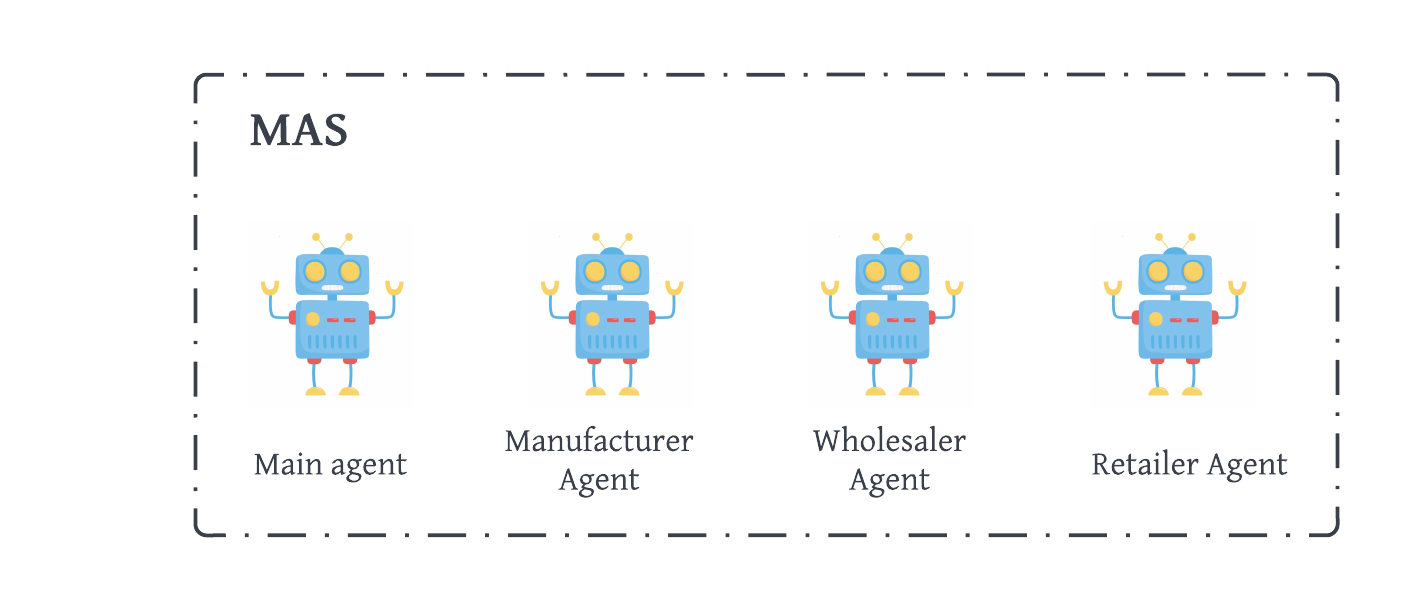
\includegraphics[width=10cm]{includes/figures/MAS.png} 
  \caption{Agents in \ac{MAS}}
  \label{Agents in MAS}
\end{figure}

\subsection{Jason interpreter built on Java}

AgentSpeak's expanded dialect has an interpreter named Jason. It implements the operational semantics of that language and offers a platform for creating \ac{MAS} with a variety of characteristics that may be altered by the user. Version 3.1 of Jason, which is the most recent version, was installed. The agents are constructed using figure  \ref{Agent Interaction} as a guide.

\vspace{.5cm}

In addition to being able to interpret the original AgentSpeak, Jason possesses a few other crucial abilities. Inter-agent communication based on speech acts and strong negation are included, allowing for the use of both closed- and open-world assumptions. Additionally, it supports creating environments (which are not normally to be programmed in AgentSpeak; in this case they are programmed in Java). It offers the ability to deploy distributed \ac{MAS} via a network (using \ac{JADE}); the user may also add other distribution infrastructures. Furthermore, it offers an \ac{IDE} in the form of an Eclipse or jEdit plugin; the \ac{IDE} has a "mind inspector" that aids with debugging.

\subsection{\ac{ASTRA} Implementation}

\ac{ASTRA} programs are divided into agent classes, which may be expanded using a multiple inheritance paradigm. Each agent class is written in a separate file with the same name as the agent class and the \texttt{.astra} extension. \ac{ASTRA} is distinct from AgentSpeak (L). Because \ac{ASTRA} applications can refer to Java classes, support for delivering fully qualified class names is required. \ac{ASTRA} programs incorporate partial plans (called plan bodies) in addition to plan rules to promote code/class resuability. \ac{ASTRA} strives to be familiar to developers who are familiar with mainstream programming languages, particularly Java.

 \vspace{.5cm}
 
Agent Programming Languages are intended to aid in the creation of MAS. Such systems are intended to have more than one agent and more than one agent type by default. Support for deploying numerous agents is given in many Agent Programming Languages via deployment files, which let the developer to define the initial community of agents to be deployed. \ac{ASTRA} does not support this; instead, you construct an agent that generates new agents. The System \ac{API} provides the essential functionality to allow this approach. In \ac{ASTRA}, coding one agent to produce another agent is extremely straightforward. You just invoke the System \ac{API}'s \texttt{createAgent(...)} operation.

\subsection{Jason interpreter built on python}

An interpreter for Jason, an agent-oriented programming language, built on Python. It can be installed in the system using \texttt{\ac{pip}}. For our implementation, we utilized agentspeak 0.1.0. Python-agentspeak is similar to Jason, except you don't need to create a \texttt{.mas2j} file to construct a multi-agent system; instead, all the agents may be called together by calling them in a \texttt{.py} file.

\section{Smart Contracts Development}

Solidity language is used to create smart contracts, while JavaScript is used for testing. The \texttt{.sol} files were compiled using Solidity v0.8.13, which also produced \texttt{.abi} and \texttt{.bin} files. The truffle tool, especially truffle v5.6.5, has been used for deployment and testing. We have used ganache v7.5.0 and ganache-UI v2.5.4 to examine state and manage chain behavior. All of the packages listed below have been obtained using node v14.0.0 (npm v6.14.4) in the table \ref{Package Version}.
    
\vspace{.5cm}

\begin{table}[h]
\small
\centering
\caption{Package Version}
\label{Package Version}
\begin{tabular}{|l| l|}
\hline
\textbf{Node Package} & \textbf{Version} \\ 
\hline\hline
web3 & 1.7.5\\ \hline
truffle & 5.6.5\\ \hline 
@truffle/contract & 4.5.22\\ \hline 
@truffle/hdwallet-provider & 2.0.13\\ \hline
dotenv & 16.0.1\\ \hline
geth & 0.4.0\\ \hline
openzeppelin & 4.7.3\\ \hline
\hline 
\end{tabular}
\end{table}

\vspace{.5cm}

Figure \ref{Activity Diagram} was used as a reference for developing smart contracts connected to supply chain. The following events were included in the supply chain: To complete the supply chain, (i) the manufacturer manufactures the product, (ii) the manufacturer packages the product, (iii) the manufacturer sells the product to the wholesaler, (iv) the wholesaler purchases the product, (v) the wholesaler receives the product, (vi) the wholesaler sells the product to the retailer, (vii) the retailer purchases the product, (viii) the retailer receives the product, and restocks his/her inventory.

\begin{figure}[h]
\centering
  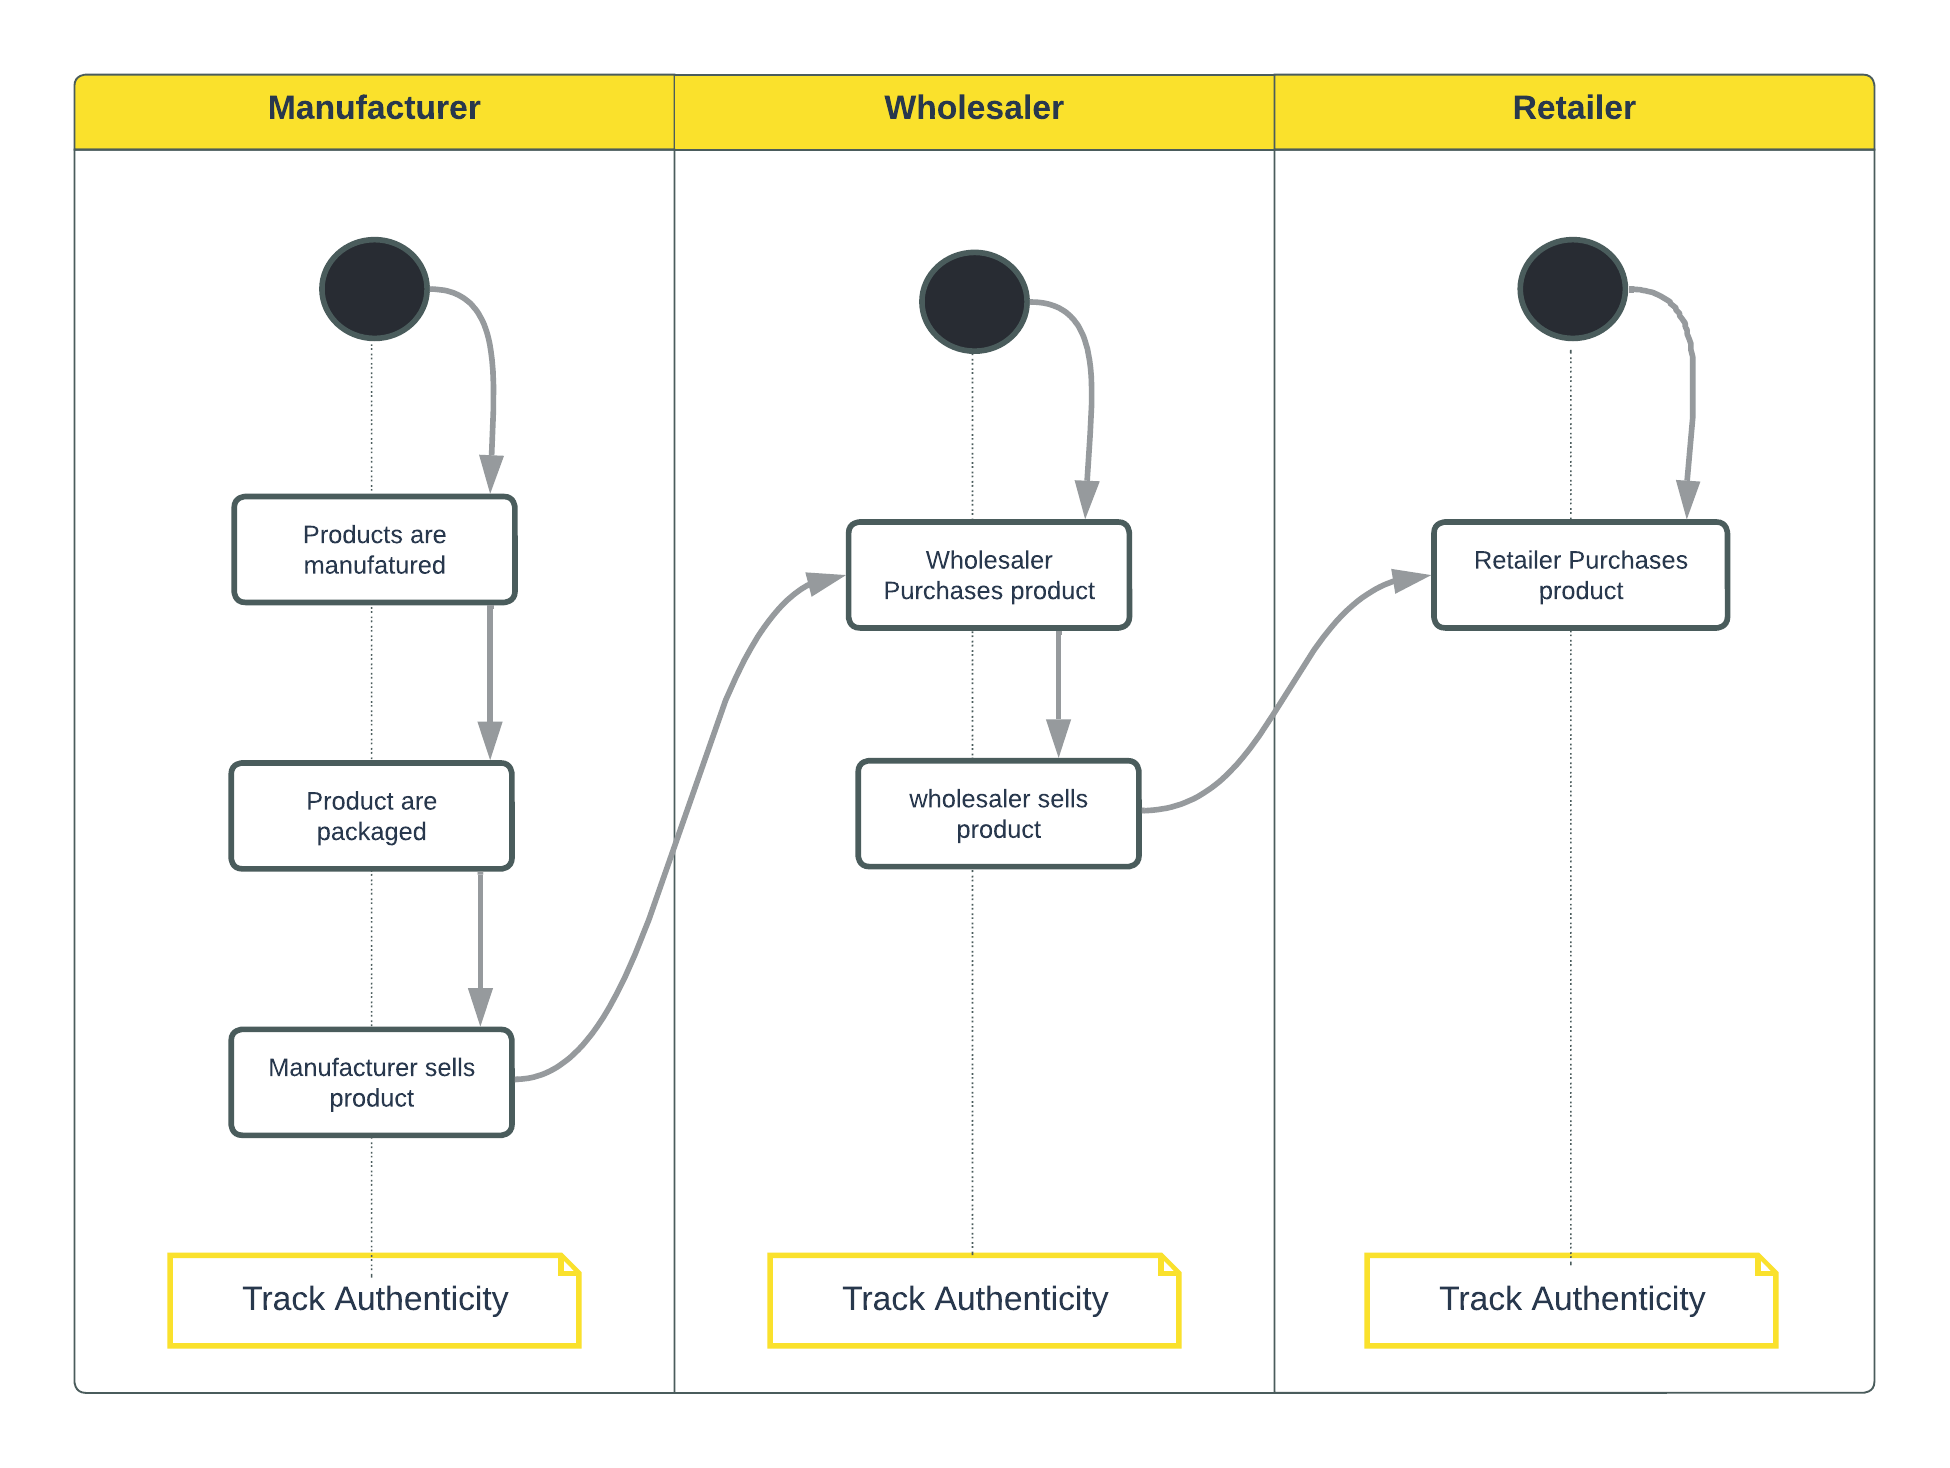
\includegraphics[width=12cm]{includes/figures/Activity Diagram.png} 
  \caption{Supply Chain Activity Diagram}
  \label{Activity Diagram}
\end{figure}

\vspace{.5cm}

The way in which files organised an classes imported using inheritance can be understand from Figure \ref{Data Model diagram}, but for the in depth understanding Figure \ref{Overall Class Diagram} should be taken into consideration.

\vspace{.5cm}
\textbf{Vyper} was also chosen to construct smart contracts, which is now one of \ac{DeFi}'s most popular languages. Vyper is a high-level programming language identical to Python. However, due to its limitations over Solidity, the proposal was subsequently abandoned.

\newpage

\begin{figure}[h]
\centering
  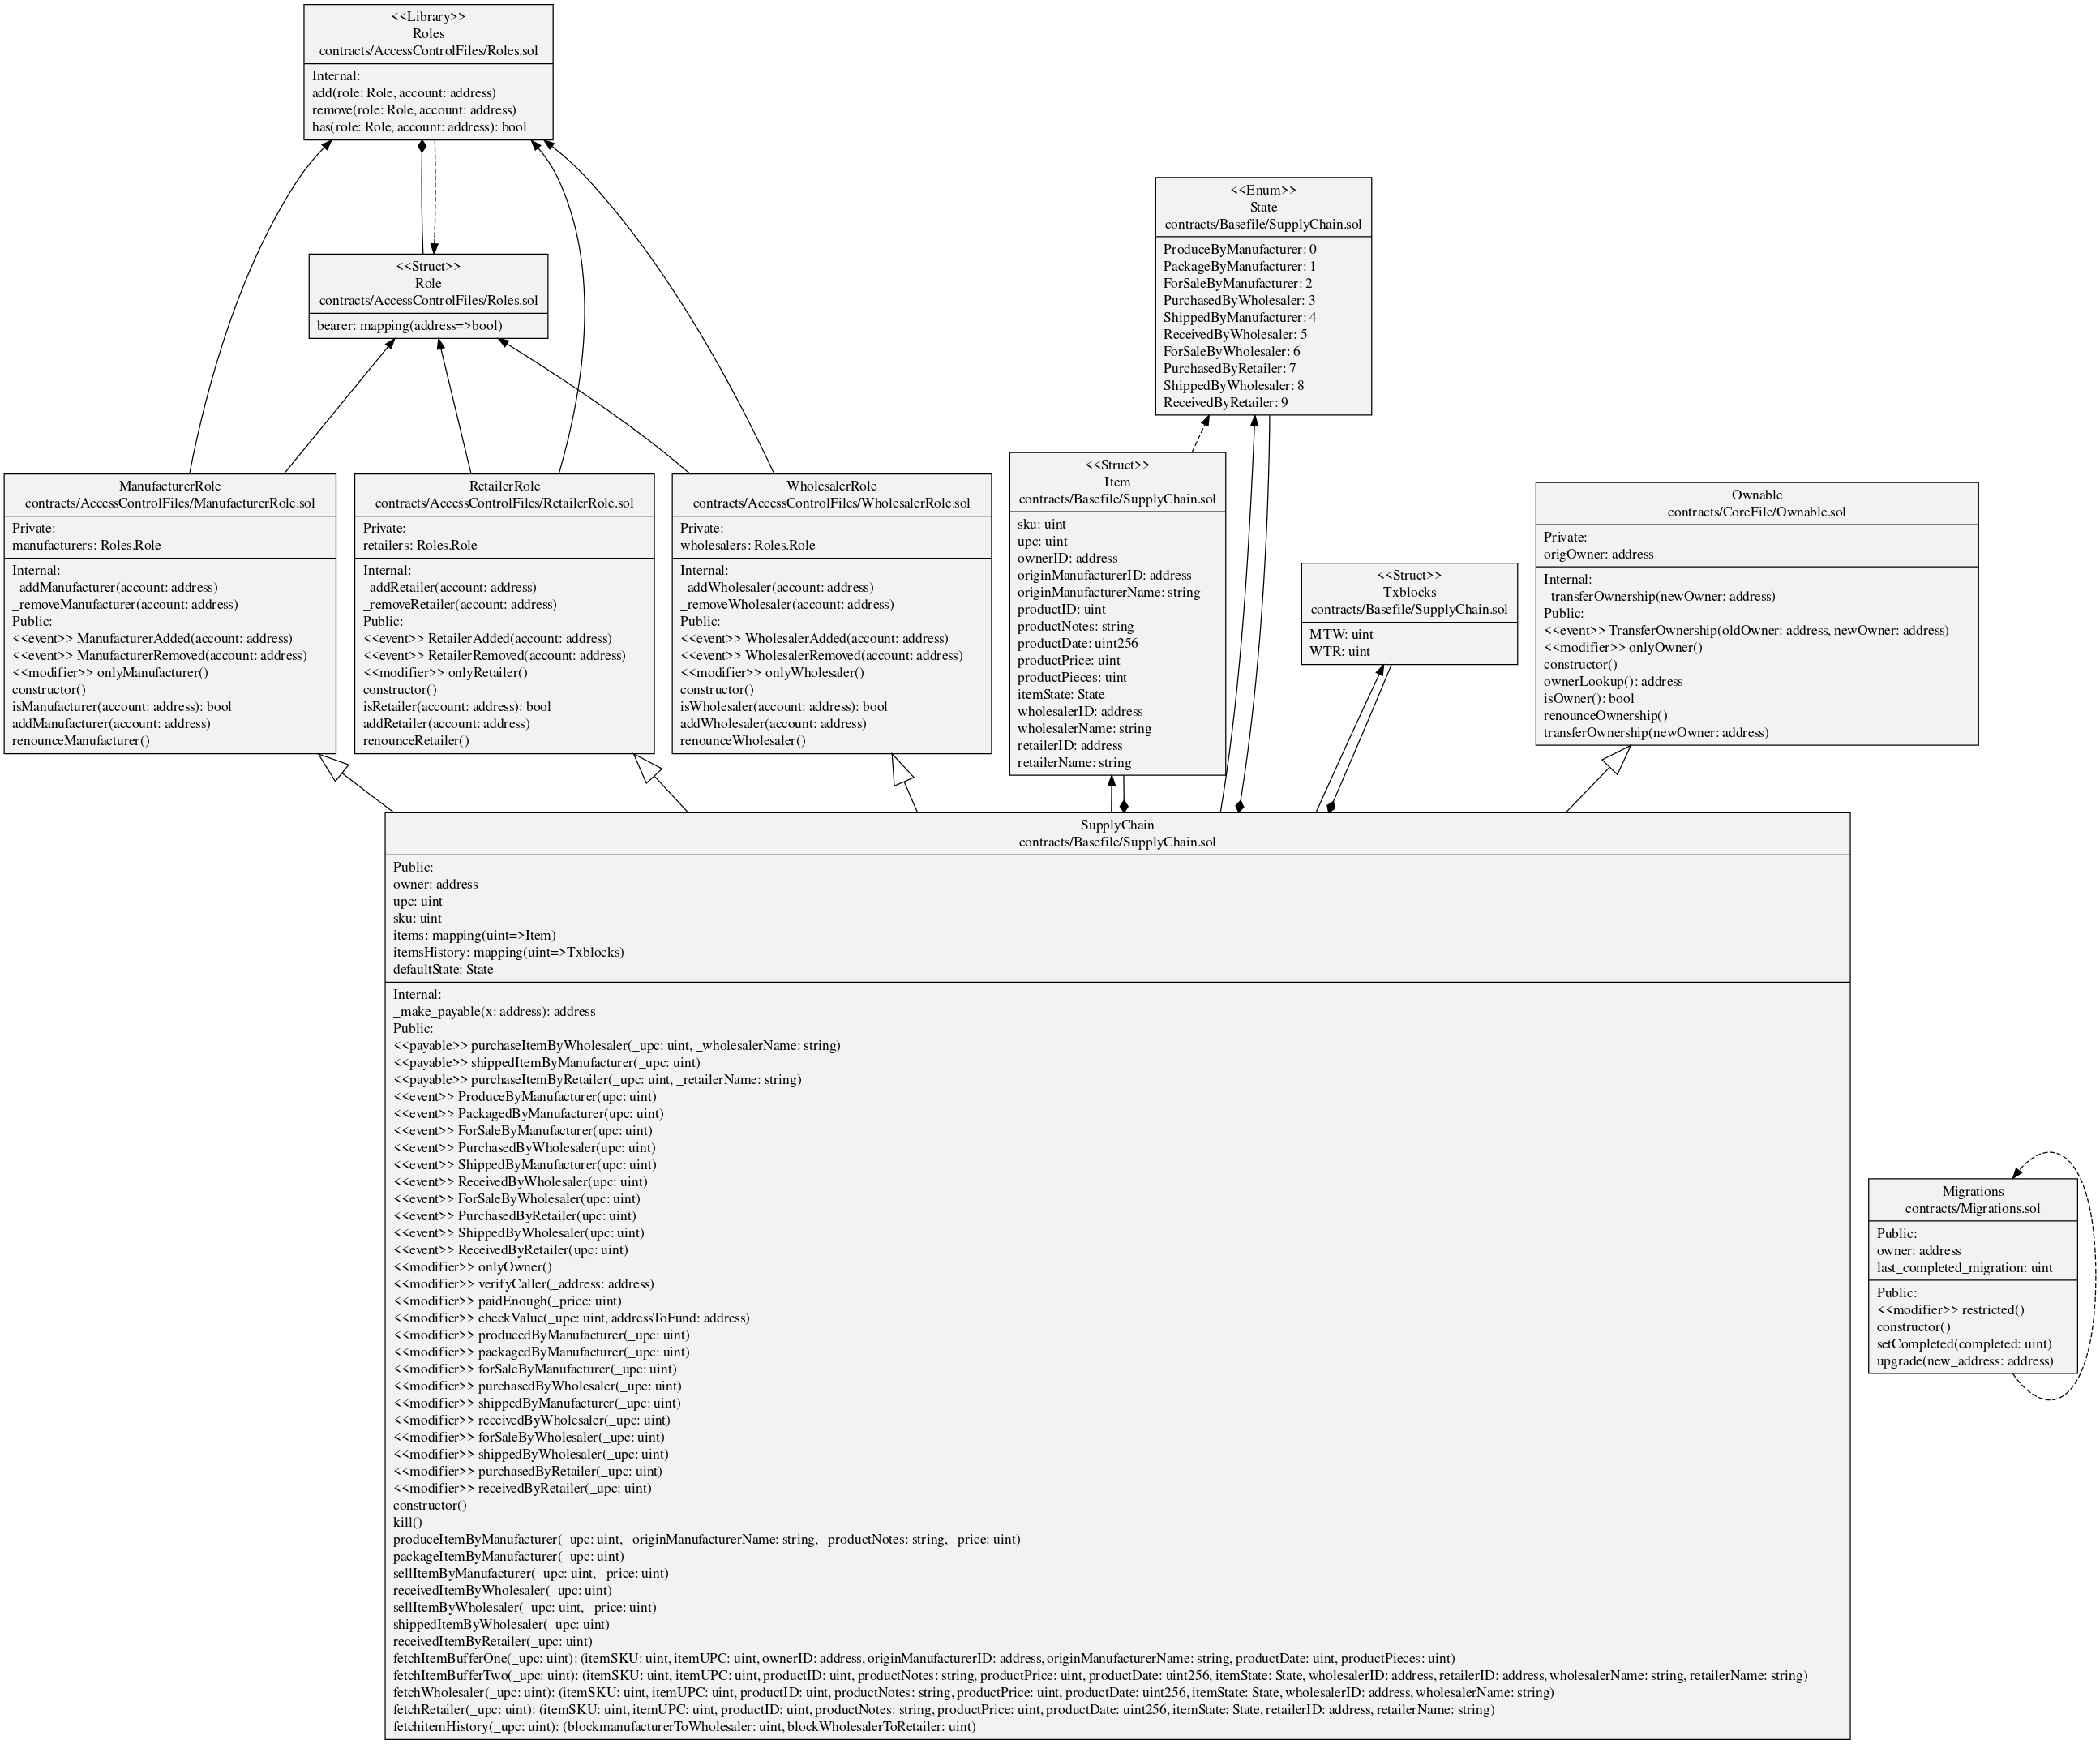
\includegraphics[width=22cm, angle=90]{includes/figures/OverallClassDiagram.png} 
  \caption{Smart Contract Class Diagram}
  \label{Overall Class Diagram}
\end{figure}

\vspace{.5cm}



\section{Integrating \ac{MAS}-\ac{BCT}}

The thesis' core premise is the integration of the two technologies, \ac{MAS} and \ac{BCT}. We have tried to integrate both the technologies using several tries by using several web3 libraries, i.e., \textit{web3.js} for JavaScript, \textit{web3.py} for Python and \textit{web3j} for Java in order to interact with Ethereum.

\subsection{Jason and Web3j}

We attempted to test each smart contract using web3js after generating them with Solidity. We considered migrating to web3j since it would be simpler as opposed to continuing to utilize Jason AgentSpeak, which is based on Java. Through the Command Line Tools tool, Web3j facilitates the development of Java smart contract function wrappers from Solidity ABI files or straight from Truffle's Contract Schema. To reveal the contract's per-network deployment address, a wrapper is "improved" and produced. When the wrapper is created, these addresses are from the truffle deployment.

\vspace{.5cm}

The plan to utilize Web3j with Jason was eventually scrapped since, in order for Jason to run \ac{MAS}, the \texttt{.mas2j} file had to be executed, and when it did, it couldn't find the \texttt{org.web3j} package. We attempted to download the jar files locally, change the version of web3j and jason, and switched from gradle to maven in order to make the program run, but the problem persisted.

\subsection{\ac{ASTRA} and Web3j}

After several attempts with web3j and Jason, we considered switching to \ac{ASTRA}, a programming language that is quite similar to Java and aims to be familiar to developers with language. A successful agent construction was followed by the same problem as with Jason when importing the web3j package.

\subsection{Jason and Web3.py}

Web3.py is a Python package that allows you to connect with Ethereum. It is often used in \ac{Dapp}s to support a number of use cases, including sending transactions, communicating with smart contracts, accessing block data, and more. The Web3.js JavaScript \ac{API} served as the foundation for the original \ac{API}, which has since expanded to meet the demands and conveniences of Python developers.

\vspace{.5cm}

Jason's Python interpreter and Web3.py worked well together. In order to communicate or convey messages from one agent to another, \texttt{.asl} files for agents were produced in Python using AgentSpeak, which is a bit different from Jason constructed using Java. Additionally, running a \texttt{.mas2j} file is not necessary for \ac{MAS} in Jason-style AgentSpeak for Python.

\subsection{Jason and Jython}

Jason AgentSpeak's smart contract development for Python and Web3py was a success. So we decided to give it another shot and try to develop it using Jython. The Jython project provides Python implementations in Java, giving Python the benefits of operating on the JVM and access to Java classes.

\vspace{.5cm}

We attempted to use Jason with Java by converting the Python code into a Java application. The creation of a Java application containing Python code was successful, but when the \texttt{.mas2j} file was executed, it was unable to import the package \texttt{org.python} , which is necessary to start the program.
	
	\chapter{Evaluation}
	\chapter{Evaluation}
This chapter focuses on reviewing all of the work completed while utilizing all of the technologies to construct the application. Prior to integrating the technologies, each technique is evaluated independently.

\section{Smart Contract Performance }

\subsection{Performance Over Test Networks}

\begin{figure}[h]
\centering
  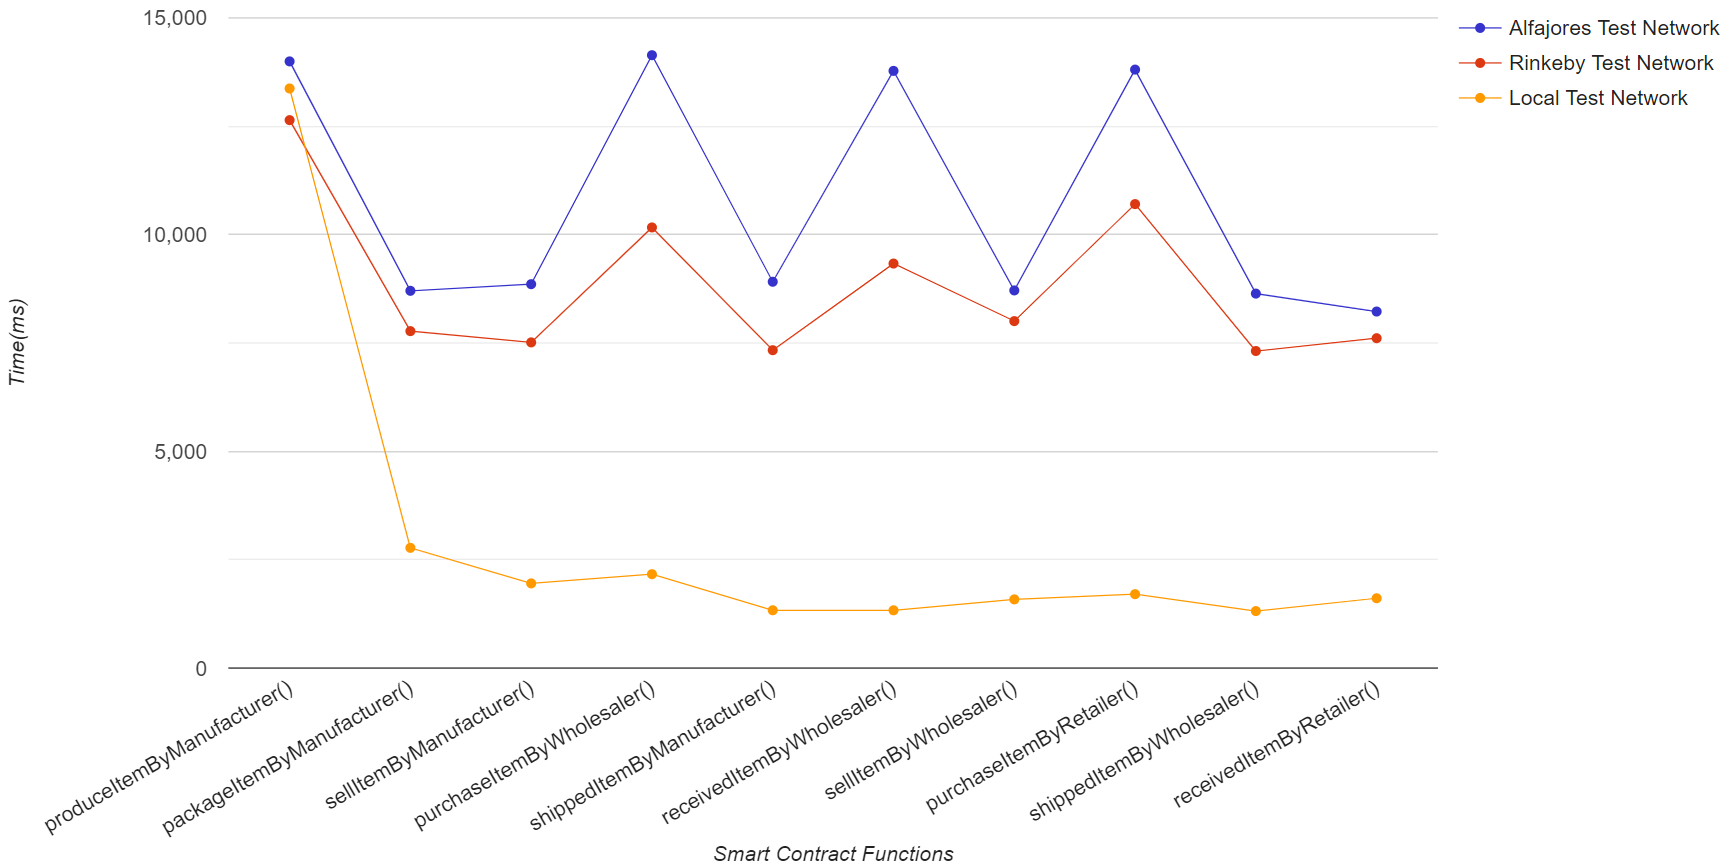
\includegraphics[width=15cm]{includes/figures/graph.png} 
  \caption{Performance across various networks}
  \label{Testing on networks}
\end{figure}

\subsection{Contract Language Comparison}

Jason's and some issue with web3 libraries gave the opportunity to switch from Solidity to Vyper and learn more about the language. Because Vyper lacks \textit{Modifiers}, \textit{Class Inheritance}, \textit{Inline Assembly}, \textit{Function Overloading}, \textit{Operator Overloading}, and \textit{Binary Fixed Point}, a thorough examination of Vyper prompted us to chose Solidity once more. The usage of the following constructs might result in confusing or challenging to comprehend code, hence they are not included.

\subsection{Incompatibility Issues}
	
	\chapter{Future Work}
	\chapter{Future Work}
	
	\chapter{Conclusion}
	\chapter{Conclusion}

In this thesis, we discussed about the \ac{MAS} and \ac{BCT}, which are well-known technologies that will likely be employed in the future in a significant supply chain sector. We provide an implementation and a sample regarding the creation of smart contracts with Jason \ac{BDI} agents, whereby the smart contracts are constructed using Solidity, the agents are developed with the Jason Python interpreter, and both are integrated with the web3.py package.
	
	
\cleardoublepage
\pagenumbering{roman}
	
	\appendix
	
	%todo: Add appendices
	\chapter{Appendix}
	
	
	% List of Abbreviations
	%todo: Include your abbreviations into includes/acronyms.tex
	\chapter*{List of Abbreviations}
\addcontentsline{toc}{chapter}{List of Abbreviations}

% ========================================================================= CALLING
% \ac{abbr.}         % default:	full at first call, short (abbr.) else
% \acs{abbr.}        % short: 	abbr.
% \acf{abbr.}        % full: 	abbreviation (abbr.)
% \acl{abbr.}        % long: 	abbreviation
%
% for plural forms, add a -p: \acp, \acsp, \acfp, \aclp

% ========================================================================= CREATION
% \acro{POSF}{Partly Open Software Family}
% \acroplural{POSF}[POSFs]{Partly Open Software Families}

\begin{acronym}[SEPSEP]
	\acro{POSF}{Partly Open Software Family}
	%B
	%C
	%D
	%E
	%F
	%G
	%H
	%I
	%J
	%K
	%L
	%M
	%N
	%O
	%P
	%Q
	%R
	%S
	%T
	%U
	%V
	%W
	%X
	%Y
	%Z
\end{acronym}

	
%%%%%%%%%%%%%%%%%%%%%%%%%%%%%%%%%%%%%%%%%%%%%%%%%%%%%%%%%%%%%%%%
% THE FOLLOWING WILL GENERATE LISTS AUTOMATICALLY
% DO NOT CHANGE THE CODE BESIDES THE LISTS' ORDER
	
	% List of Definitions
	\renewcommand{\listtheoremname}{List of Definitions}
	\listoftheorems[ignoreall,show={definition}]
	% List of Figures
	\listoffigures
	% List of Tables
	\listoftables
	% List of Listings
	\renewcommand{\lstlistlistingname}{List of \lstlistingname s}
	\lstlistoflistings	
	% List of Formulas
	\renewcommand{\listtheoremname}{List of Formulas}
	\listoftheorems[ignoreall,show={formula}]
	% Bibliography
	\printbibliography %\printbibliography[heading=bibintoc] if ToC entry desired

\end{document}
